
\documentclass[krantz1,ChapterTOCs, book]{krantz}
\usepackage{fixltx2e,fix-cm}
\usepackage{amssymb}
\usepackage{amsmath}
\usepackage{graphicx}
\usepackage{subfigure}
\usepackage{makeidx}
\usepackage{multicol}
\usepackage{hyperref}
\usepackage{graphicx}
\usepackage{listings}
\usepackage[utf8]{inputenc}

\frenchspacing
\tolerance=5000

\makeindex

\newtheorem{theorem}{Theorem}
\newtheorem{exercise}{Exercise}[chapter]
\newtheorem{example}{Example}
\newtheorem{definition}{Definition}
\newtheorem{proof}{Proof}
 %place custom commands and macros here

\begin{document}

\frontmatter

\title{STEM Outreach Activities... 
}
\author{Scott Turner}
\begin{figure}
    \centering
    \includegraphics[width=11cm]{chapters/DALL·E 2023-03-06 14.40.17 - Manga style robot teaching.png}
\end{figure}
\maketitle

%\cleardoublepage
\thispagestyle{empty}
\vspace*{\stretch{1}}
\begin{center}
\Large\itshape
To my dog\\
and my cat.
\end{center}
\vspace{\stretch{2}}
%\cleardoublepage
\setcounter{page}{7} %previous pages will be reserved for frontmatter to be added in later.
\tableofcontents
%\chapter*{Foreword}
I am delighted to introduce the first book on Multimedia Data Mining.  When I came to know about this book project undertaken by two of the most active young researchers in the field, I was pleased that this book is coming in early stage of a field that will need it more than most fields do.  In most emerging research fields, a book can play a significant role in bringing some maturity to the field.  Research fields advance through research papers.  In research papers, however, only a limited perspective could be provided about the field, its application potential, and the techniques required and already developed in the field.  A book gives such a chance.  I liked the idea that there will be a book that will try to unify the field by bringing in disparate topics already available in several papers that are not easy to find and understand.  I was supportive of this book project even before I had seen any material on it.  The project was a brilliant and a bold idea by two active researchers.  Now that I have it on my screen, it appears to be even a better idea.  

Multimedia started gaining recognition in 1990s as a field.  Processing, storage, communication, and capture and display technologies had advanced enough that researchers and technologists started building approaches to combine information in multiple types of signals such as audio, images, video, and  text.  Multimedia computing and communication techniques recognize correlated information in multiple sources as well as insufficiency of information in any individual source.    By properly selecting sources to provide complementary information, such systems aspire, much like human perception system, to create a holistic picture of a situation using only partial information from separate sources.

Data mining is a direct outgrowth of progress in data storage and processing speeds.  When it became possible to store large volume of data and run different statistical computations to explore all possible and even unlikely correlations among data, the field of data mining was born.  Data mining allowed people to hypothesize relationships among data entities and explore support for those.  This field has been put to applications in many diverse domains and keeps getting more applications.  In fact many new fields are direct outgrowth of data mining and it is likely to become a powerful computational tool.\vadjust{\vfill\pagebreak}



%\chapter*{Preface}
Approximately 17 million people in the USA (6{\%} of the
population) and 140 million people worldwide (this number is
expected to rise to almost 300 million by the year 2025) suffer
from \textit{diabetes mellitus}. Currently, there a few dozens of
commercialised devices for detecting blood glucose levels [1].
However, most of them are invasive. The development of a
noninvasive method would considerably improve the quality of life
for diabetic patients, facilitate their compliance for glucose
monitoring, and reduce complications and mortality associated with
this disease. Noninvasive and continuous monitoring of glucose
concentration in blood and tissues is one of the most challenging
and exciting applications of optics in medicine. The major
difficulty in development and clinical application of optical
noninvasive blood glucose sensors is associated with very low
signal produced by glucose molecules. This results in low
sensitivity and specificity of glucose monitoring by optical
methods and needs a lot of efforts to overcome this difficulty.

A wide range of optical technologies have been designed in
attempts to develop robust noninvasive methods for glucose
sensing. The methods include infrared absorption, near-infrared
scattering, Raman, fluorescent, and thermal gradient
spectroscopies, as well as polarimetric, polarization
heterodyning, photonic crystal, optoacoustic, optothermal, and
optical coherence tomography (OCT) techniques [1-31].

For example, the polarimetric quantification of glucose is based
on the phenomenon of optical rotatory dispersion, whereby a chiral
molecule in an aqueous solution rotates the plane of linearly
polarized light passing through the solution. The angle of
rotation depends linearly on the concentration of the chiral
species, the pathlength through the sample, and the molecule
specific rotation. However, polarization sensitive optical
technique makes it difficult to measure \textit{in vivo} glucose
concentration in blood through the skin because of the strong
light scattering which causes light depolarization. For this
reason, the anterior chamber of the eye has been suggested as a
sight well suited for polarimetric measurements, since scattering
in the eye is generally very low compared to that in other
tissues, and a high correlation exists between the glucose in the
blood and in the aqueous humor. The high accuracy of anterior eye
chamber measurements is also due to the low concentration of
optically active aqueous proteins within the aqueous humor.

On the other hand, the concept of noninvasive blood glucose
sensing using the scattering properties of blood and tissues as an
alternative to spectral absorption and polarization methods for
monitoring of physiological glucose concentrations in diabetic
patients has been under intensive discussion for the last decade.
Many of the considered  effects, such as changing of the size,
refractive index, packing, and aggregation of RBC under glucose
variation, are important for glucose monitoring in diabetic
patients. Indeed, at physiological concentrations of glucose,
ranging from 40 to 400 mg/dl, the role of some of the effects may
be modified, and some other effects, such as glucose penetration
inside the RBC and the followed hemoglobin glycation, may be
important [30-32].

Noninvasive determination of glucose was attempted using light
scattering of skin tissue components measured by a
spatially-resolved diffuse reflectance or NIR fre\-quen\-cy-domain
reflectance techniques. Both approaches are based on change in
glucose concentration, which affects the refractive index mismatch
between the interstitial fluid and tissue fibers, and hence
reduces scattering coefficient. A glucose clamp experiment showed
that reduced scattering coefficient measured in the visible range
qualitatively tracked changes in blood glucose concentration for
the volunteer with diabetes studied.




\listoffigures
%%%\twocolumn
\chapter*{Contributors}

\begin{multicols}{2}
\contributor{Michael Aftosmis}{NASA Ames Research Center}{Moffett Field, California}

\contributor{Pratul K. Agarwal}{Oak Ridge National Laboratory}{Oak Ridge, Tennessee}

\contributor{Sadaf R. Alam}{Oak Ridge National Laboratory}{Oak Ridge, Tennessee}

\contributor{Gabrielle Allen}{Louisiana State University}{Baton Rouge, Louisiana}

\contributor{Martin Sandve Aln{\ae}s}{Simula Research Laboratory and University of Oslo, Norway}{Norway}

\contributor{Steven F. Ashby} {Lawrence Livermore National Laboratory}{Livermore, California}

\contributor{David A. Bader} {Georgia Institute of Technology}{Atlanta, Georgia}

\contributor{Benjamin Bergen} {Los Alamos National Laboratory}{Los Alamos, New Mexico}

\contributor{Jonathan W. Berry} {Sandia National Laboratories}{Albuquerque, New Mexico}

\contributor{Martin Berzins}{University of Utah}{Salt Lake City, Utah}

\contributor{Abhinav Bhatele}{University of Illinois}{Urbana-Champaign, Illinois}

\contributor{Christian Bischof} {RWTH Aachen University}{Germany}

\contributor{Rupak Biswas} {NASA Ames Research Center}{Moffett Field, California}\vspace*{5pt}

\contributor{Eric Bohm} {University of Illinois}{Urbana-Champaign, Illinois}\vspace*{5pt}

\contributor{James Bordner} {University of California, San Diego}{San Diego, California}\vspace*{5pt}

\contributor{George Bosilca} {University of Tennessee}{Knoxville, Tennessee}\vspace*{5pt}

\contributor{Greg L. Bryan} {Columbia University}{New York, New York}\vspace*{5pt}

\contributor{Marian Bubak} {AGH University of Science and Technology}{
Krak{\'o}w, Poland}\vspace*{5pt}

\contributor{Andrew Canning}{Lawrence Berkeley National
Laboratory}{Berkeley, California}

\contributor{Jonathan Carter} {Lawrence Berkeley National
Laboratory}{Berkeley, California}

\contributor{Zizhong Chen} {Jacksonville State University}{Jacksonville,
Alabama}

\contributor{Joseph R. Crobak} {Rutgers, The State University of New
Jersey}{Piscataway, New Jersey}

\contributor{Roxana E. Diaconescu} {Yahoo! Inc.}{Burbank, California}

\contributor{Peter Diener}
{Louisiana State University}{Baton Rouge, Louisiana}

\contributor{Jack J. Dongarra} {University of Tennessee, Knoxville, 
Oak Ridge National Laboratory, and}{University of Manchester}

\contributor{John B. Drake} {Oak Ridge National Laboratory}{Oak Ridge,
Tennessee}

\contributor{Kelvin K. Droegemeier} {University of Oklahoma}{Norman,
Oklahoma}

\contributor{St{\'e}phane Ethier} {Princeton University}{Princeton, New
Jersey}

\contributor{Christoph Freundl}
{Friedrich--Alexander--Universit{\"a}t}{Erlangen, Germany}

\contributor{Karl F{\"u}rlinger} {University of Tennessee}{Knoxville,
Tennessee}

\contributor{Al Geist} {Oak Ridge National Laboratory}{Oak Ridge,
Tennessee}

\contributor{Michael Gerndt} {Technische Universit{\"a}t
M{\"u}nchen}{Munich, Germany}

\contributor{Tom Goodale}
{Louisiana State University}{Baton Rouge, Louisiana}

\contributor{Tobias Gradl}
{Friedrich--Alexander--Universit{\"a}t}{Erlangen, Germany}

\contributor{William D. Gropp} {Argonne National Laboratory}{Argonne,
Illinois}

\contributor{Robert Harkness} {University of California, San
Diego}{San Diego, California}

\contributor{Albert Hartono} {Ohio State University}{Columbus, Ohio}

\contributor{Thomas C. Henderson} {University of Utah}{Salt Lake City,
Utah}

\contributor{Bruce A. Hendrickson} {Sandia National
Laboratories}{Albuquerque, New Mexico}

\contributor{Alfons G. Hoekstra} {University of Amsterdam}{Amsterdam,
The Netherlands}

\contributor{Philip W. Jones} {Los Alamos National Laboratory}{Los
Alamos, New Mexico}

\contributor{Laxmikant Kal{\'e}} {University of
Illinois}{Urbana-Champaign, Illinois}

\contributor{Shoaib Kamil} {Lawrence Berkeley National
Laboratory}{Berkeley, California}

\contributor{Cetin Kiris} {NASA Ames Research Center}{Moffett Field,
California}

\contributor{Uwe K{\"u}ster} {University of Stuttgart}{Stuttgart,
Germany}

\contributor{Julien Langou} {University of Colorado}{Denver, Colorado}

\contributor{Hans Petter Langtangen}
{Simula Research Laboratory and}{University of Oslo, Norway}

\contributor{Michael Lijewski} {Lawrence Berkeley National
Laboratory}{Berkeley, California}

\contributor{Anders Logg}
{Simula Research Laboratory and}{University of Oslo, Norway}

\contributor{Justin Luitjens} {University of Utah}{Salt Lake City, Utah}

\contributor{Kamesh Madduri} {Georgia Institute of Technology}{Atlanta,
Georgia}

\contributor{Kent-Andre Mardal}
{Simula Research Laboratory and}{University of Oslo, Norway}

\contributor{Satoshi Matsuoka} {Tokyo Institute of Technology}{Tokyo,
Japan}

\contributor{John M. May} {Lawrence Livermore National
Laboratory}{Livermore, California}

\contributor{Celso L. Mendes} {University of Illinois}{Urbana-Champaign,
Illinois}

\contributor{Dieter an Mey} {RWTH Aachen University}{Germany}

\contributor{Tetsu Narumi} {Keio University}{Japan}

\contributor{Michael L. Norman} {University of California, San
Diego}{San Diego, California}

\contributor{Boyana Norris} {Argonne National Laboratory}{Argonne,
Illinois}

\contributor{Yousuke Ohno} {Institute of Physical and Chemical Research
(RIKEN)}{Kanagawa, Japan}

\contributor{Leonid Oliker} {Lawrence Berkeley National
Laboratory}{Berkeley, California}

\contributor{Brian O'Shea} {Los Alamos National Laboratory}{Los Alamos,
New Mexico}

\contributor{Christian D. Ott}
{University of Arizona}{Tucson, Arizona}

\contributor{James C. Phillips} {University of
Illinois}{Urbana-Champaign, Illinois}

\contributor{Simon Portegies Zwart} {University of
Amsterdam,}{Amsterdam, The Netherlands}

\contributor{Thomas Radke}
{Albert-Einstein-Institut}{Golm, Germany}

\contributor{Michael Resch} {University of Stuttgart}{Stuttgart,
Germany}

\contributor{Daniel Reynolds} {University of California, San Diego}{San
Diego, California}

\contributor{Ulrich R{\"u}de}
{Friedrich--Alexander--Universit{\"a}t}{Erlangen, Germany}

\contributor{Samuel Sarholz}
{RWTH Aachen University}{Germany}

\contributor{Erik Schnetter}
{Louisiana State University}{Baton Rouge, Louisiana}

\contributor{Klaus Schulten} {University of Illinois}{Urbana-Champaign,
Illinois}

\contributor{Edward Seidel}
{Louisiana State University}{Baton Rouge, Louisiana}

\contributor{John Shalf} {Lawrence Berkeley National
Laboratory}{Berkeley, California}

\contributor{Bo-Wen Shen} {NASA Goddard Space Flight Center}{Greenbelt,
Maryland}

\contributor{Ola Skavhaug}
{Simula Research Laboratory and}{University of Oslo, Norway}

\contributor{Peter M.A. Sloot} {University of Amsterdam}{Amsterdam, The
Netherlands}

\contributor{Erich Strohmaier} {Lawrence Berkeley National
Laboratory}{Berkeley, California}

\contributor{Makoto Taiji} {Institute of Physical and Chemical Research
(RIKEN)}{Kanagawa, Japan}

\contributor{Christian Terboven}
{RWTH Aachen University,}{Germany}

\contributor{Mariana Vertenstein} {National Center for Atmospheric
Research}{Boulder, Colorado}

\contributor{Rick Wagner} {University of California, San Diego}{San
Diego, California}

\contributor{Daniel Weber} {University of Oklahoma}{Norman, Oklahoma}

\contributor{James B. White, III} {Oak Ridge National Laboratory}{Oak
Ridge, Tennessee}

\contributor{Terry Wilmarth} {University of Illinois}{Urbana-Champaign,
Illinois}

\end{multicols}
%\chapter*{Symbols}
\begin{symbollist}{000000}
\symbolentry{$\alpha$}{To solve the generator maintenance scheduling, in the  past, several mathematical techniques have  been applied.}
\symbolentry{$\sigma^2$}{These include integer programming, integer linear programming, dynamic programming, branch and bound etc.}
\symbolentry{$\sum$}{Several heuristic search algorithms have also been developed. In recent years expert systems,}
\symbolentry{$abc$}{fuzzy approaches, simulated annealing and genetic algorithms have also been tested.}
\symbolentry{$\theta\sqrt{abc}$}{This paper presents a survey of the literature}
\symbolentry{$\zeta$}{ over the past fifteen years in the generator}
\symbolentry{$\partial$}{maintenance scheduling. The objective is to}
\symbolentry{sdf}{present a clear picture of the available recent literature}
\symbolentry{ewq}{of the problem, the constraints and the other aspects of}
\symbolentry{bvcn}{the generator maintenance schedule.}
\end{symbollist}

\mainmatter
\part{Web-based VR and AR}
\documentclass[krantz1,ChapterTOCs, book]{krantz}
\usepackage{fixltx2e,fix-cm}
\usepackage{amssymb}
\usepackage{amsmath}
\usepackage{graphicx}
\usepackage{subfigure}
\usepackage{makeidx}
\usepackage{multicol}
\usepackage{hyperref}
\usepackage{graphicx}
\usepackage{listings}
\usepackage[utf8]{inputenc}

\frenchspacing
\tolerance=5000

\makeindex

\newtheorem{theorem}{Theorem}
\newtheorem{exercise}{Exercise}[chapter]
\newtheorem{example}{Example}
\newtheorem{definition}{Definition}
\newtheorem{proof}{Proof}
 %place custom commands and macros here

\begin{document}

\frontmatter

\title{STEM Outreach Activities... 
}
\author{Scott Turner}
\begin{figure}
    \centering
    \includegraphics[width=11cm]{chapters/DALL·E 2023-03-06 14.40.17 - Manga style robot teaching.png}
\end{figure}
\maketitle

%\cleardoublepage
\thispagestyle{empty}
\vspace*{\stretch{1}}
\begin{center}
\Large\itshape
To my dog\\
and my cat.
\end{center}
\vspace{\stretch{2}}
%\cleardoublepage
\setcounter{page}{7} %previous pages will be reserved for frontmatter to be added in later.
\tableofcontents
%\chapter*{Foreword}
I am delighted to introduce the first book on Multimedia Data Mining.  When I came to know about this book project undertaken by two of the most active young researchers in the field, I was pleased that this book is coming in early stage of a field that will need it more than most fields do.  In most emerging research fields, a book can play a significant role in bringing some maturity to the field.  Research fields advance through research papers.  In research papers, however, only a limited perspective could be provided about the field, its application potential, and the techniques required and already developed in the field.  A book gives such a chance.  I liked the idea that there will be a book that will try to unify the field by bringing in disparate topics already available in several papers that are not easy to find and understand.  I was supportive of this book project even before I had seen any material on it.  The project was a brilliant and a bold idea by two active researchers.  Now that I have it on my screen, it appears to be even a better idea.  

Multimedia started gaining recognition in 1990s as a field.  Processing, storage, communication, and capture and display technologies had advanced enough that researchers and technologists started building approaches to combine information in multiple types of signals such as audio, images, video, and  text.  Multimedia computing and communication techniques recognize correlated information in multiple sources as well as insufficiency of information in any individual source.    By properly selecting sources to provide complementary information, such systems aspire, much like human perception system, to create a holistic picture of a situation using only partial information from separate sources.

Data mining is a direct outgrowth of progress in data storage and processing speeds.  When it became possible to store large volume of data and run different statistical computations to explore all possible and even unlikely correlations among data, the field of data mining was born.  Data mining allowed people to hypothesize relationships among data entities and explore support for those.  This field has been put to applications in many diverse domains and keeps getting more applications.  In fact many new fields are direct outgrowth of data mining and it is likely to become a powerful computational tool.\vadjust{\vfill\pagebreak}



%\chapter*{Preface}
Approximately 17 million people in the USA (6{\%} of the
population) and 140 million people worldwide (this number is
expected to rise to almost 300 million by the year 2025) suffer
from \textit{diabetes mellitus}. Currently, there a few dozens of
commercialised devices for detecting blood glucose levels [1].
However, most of them are invasive. The development of a
noninvasive method would considerably improve the quality of life
for diabetic patients, facilitate their compliance for glucose
monitoring, and reduce complications and mortality associated with
this disease. Noninvasive and continuous monitoring of glucose
concentration in blood and tissues is one of the most challenging
and exciting applications of optics in medicine. The major
difficulty in development and clinical application of optical
noninvasive blood glucose sensors is associated with very low
signal produced by glucose molecules. This results in low
sensitivity and specificity of glucose monitoring by optical
methods and needs a lot of efforts to overcome this difficulty.

A wide range of optical technologies have been designed in
attempts to develop robust noninvasive methods for glucose
sensing. The methods include infrared absorption, near-infrared
scattering, Raman, fluorescent, and thermal gradient
spectroscopies, as well as polarimetric, polarization
heterodyning, photonic crystal, optoacoustic, optothermal, and
optical coherence tomography (OCT) techniques [1-31].

For example, the polarimetric quantification of glucose is based
on the phenomenon of optical rotatory dispersion, whereby a chiral
molecule in an aqueous solution rotates the plane of linearly
polarized light passing through the solution. The angle of
rotation depends linearly on the concentration of the chiral
species, the pathlength through the sample, and the molecule
specific rotation. However, polarization sensitive optical
technique makes it difficult to measure \textit{in vivo} glucose
concentration in blood through the skin because of the strong
light scattering which causes light depolarization. For this
reason, the anterior chamber of the eye has been suggested as a
sight well suited for polarimetric measurements, since scattering
in the eye is generally very low compared to that in other
tissues, and a high correlation exists between the glucose in the
blood and in the aqueous humor. The high accuracy of anterior eye
chamber measurements is also due to the low concentration of
optically active aqueous proteins within the aqueous humor.

On the other hand, the concept of noninvasive blood glucose
sensing using the scattering properties of blood and tissues as an
alternative to spectral absorption and polarization methods for
monitoring of physiological glucose concentrations in diabetic
patients has been under intensive discussion for the last decade.
Many of the considered  effects, such as changing of the size,
refractive index, packing, and aggregation of RBC under glucose
variation, are important for glucose monitoring in diabetic
patients. Indeed, at physiological concentrations of glucose,
ranging from 40 to 400 mg/dl, the role of some of the effects may
be modified, and some other effects, such as glucose penetration
inside the RBC and the followed hemoglobin glycation, may be
important [30-32].

Noninvasive determination of glucose was attempted using light
scattering of skin tissue components measured by a
spatially-resolved diffuse reflectance or NIR fre\-quen\-cy-domain
reflectance techniques. Both approaches are based on change in
glucose concentration, which affects the refractive index mismatch
between the interstitial fluid and tissue fibers, and hence
reduces scattering coefficient. A glucose clamp experiment showed
that reduced scattering coefficient measured in the visible range
qualitatively tracked changes in blood glucose concentration for
the volunteer with diabetes studied.




\listoffigures
%%%\twocolumn
\chapter*{Contributors}

\begin{multicols}{2}
\contributor{Michael Aftosmis}{NASA Ames Research Center}{Moffett Field, California}

\contributor{Pratul K. Agarwal}{Oak Ridge National Laboratory}{Oak Ridge, Tennessee}

\contributor{Sadaf R. Alam}{Oak Ridge National Laboratory}{Oak Ridge, Tennessee}

\contributor{Gabrielle Allen}{Louisiana State University}{Baton Rouge, Louisiana}

\contributor{Martin Sandve Aln{\ae}s}{Simula Research Laboratory and University of Oslo, Norway}{Norway}

\contributor{Steven F. Ashby} {Lawrence Livermore National Laboratory}{Livermore, California}

\contributor{David A. Bader} {Georgia Institute of Technology}{Atlanta, Georgia}

\contributor{Benjamin Bergen} {Los Alamos National Laboratory}{Los Alamos, New Mexico}

\contributor{Jonathan W. Berry} {Sandia National Laboratories}{Albuquerque, New Mexico}

\contributor{Martin Berzins}{University of Utah}{Salt Lake City, Utah}

\contributor{Abhinav Bhatele}{University of Illinois}{Urbana-Champaign, Illinois}

\contributor{Christian Bischof} {RWTH Aachen University}{Germany}

\contributor{Rupak Biswas} {NASA Ames Research Center}{Moffett Field, California}\vspace*{5pt}

\contributor{Eric Bohm} {University of Illinois}{Urbana-Champaign, Illinois}\vspace*{5pt}

\contributor{James Bordner} {University of California, San Diego}{San Diego, California}\vspace*{5pt}

\contributor{George Bosilca} {University of Tennessee}{Knoxville, Tennessee}\vspace*{5pt}

\contributor{Greg L. Bryan} {Columbia University}{New York, New York}\vspace*{5pt}

\contributor{Marian Bubak} {AGH University of Science and Technology}{
Krak{\'o}w, Poland}\vspace*{5pt}

\contributor{Andrew Canning}{Lawrence Berkeley National
Laboratory}{Berkeley, California}

\contributor{Jonathan Carter} {Lawrence Berkeley National
Laboratory}{Berkeley, California}

\contributor{Zizhong Chen} {Jacksonville State University}{Jacksonville,
Alabama}

\contributor{Joseph R. Crobak} {Rutgers, The State University of New
Jersey}{Piscataway, New Jersey}

\contributor{Roxana E. Diaconescu} {Yahoo! Inc.}{Burbank, California}

\contributor{Peter Diener}
{Louisiana State University}{Baton Rouge, Louisiana}

\contributor{Jack J. Dongarra} {University of Tennessee, Knoxville, 
Oak Ridge National Laboratory, and}{University of Manchester}

\contributor{John B. Drake} {Oak Ridge National Laboratory}{Oak Ridge,
Tennessee}

\contributor{Kelvin K. Droegemeier} {University of Oklahoma}{Norman,
Oklahoma}

\contributor{St{\'e}phane Ethier} {Princeton University}{Princeton, New
Jersey}

\contributor{Christoph Freundl}
{Friedrich--Alexander--Universit{\"a}t}{Erlangen, Germany}

\contributor{Karl F{\"u}rlinger} {University of Tennessee}{Knoxville,
Tennessee}

\contributor{Al Geist} {Oak Ridge National Laboratory}{Oak Ridge,
Tennessee}

\contributor{Michael Gerndt} {Technische Universit{\"a}t
M{\"u}nchen}{Munich, Germany}

\contributor{Tom Goodale}
{Louisiana State University}{Baton Rouge, Louisiana}

\contributor{Tobias Gradl}
{Friedrich--Alexander--Universit{\"a}t}{Erlangen, Germany}

\contributor{William D. Gropp} {Argonne National Laboratory}{Argonne,
Illinois}

\contributor{Robert Harkness} {University of California, San
Diego}{San Diego, California}

\contributor{Albert Hartono} {Ohio State University}{Columbus, Ohio}

\contributor{Thomas C. Henderson} {University of Utah}{Salt Lake City,
Utah}

\contributor{Bruce A. Hendrickson} {Sandia National
Laboratories}{Albuquerque, New Mexico}

\contributor{Alfons G. Hoekstra} {University of Amsterdam}{Amsterdam,
The Netherlands}

\contributor{Philip W. Jones} {Los Alamos National Laboratory}{Los
Alamos, New Mexico}

\contributor{Laxmikant Kal{\'e}} {University of
Illinois}{Urbana-Champaign, Illinois}

\contributor{Shoaib Kamil} {Lawrence Berkeley National
Laboratory}{Berkeley, California}

\contributor{Cetin Kiris} {NASA Ames Research Center}{Moffett Field,
California}

\contributor{Uwe K{\"u}ster} {University of Stuttgart}{Stuttgart,
Germany}

\contributor{Julien Langou} {University of Colorado}{Denver, Colorado}

\contributor{Hans Petter Langtangen}
{Simula Research Laboratory and}{University of Oslo, Norway}

\contributor{Michael Lijewski} {Lawrence Berkeley National
Laboratory}{Berkeley, California}

\contributor{Anders Logg}
{Simula Research Laboratory and}{University of Oslo, Norway}

\contributor{Justin Luitjens} {University of Utah}{Salt Lake City, Utah}

\contributor{Kamesh Madduri} {Georgia Institute of Technology}{Atlanta,
Georgia}

\contributor{Kent-Andre Mardal}
{Simula Research Laboratory and}{University of Oslo, Norway}

\contributor{Satoshi Matsuoka} {Tokyo Institute of Technology}{Tokyo,
Japan}

\contributor{John M. May} {Lawrence Livermore National
Laboratory}{Livermore, California}

\contributor{Celso L. Mendes} {University of Illinois}{Urbana-Champaign,
Illinois}

\contributor{Dieter an Mey} {RWTH Aachen University}{Germany}

\contributor{Tetsu Narumi} {Keio University}{Japan}

\contributor{Michael L. Norman} {University of California, San
Diego}{San Diego, California}

\contributor{Boyana Norris} {Argonne National Laboratory}{Argonne,
Illinois}

\contributor{Yousuke Ohno} {Institute of Physical and Chemical Research
(RIKEN)}{Kanagawa, Japan}

\contributor{Leonid Oliker} {Lawrence Berkeley National
Laboratory}{Berkeley, California}

\contributor{Brian O'Shea} {Los Alamos National Laboratory}{Los Alamos,
New Mexico}

\contributor{Christian D. Ott}
{University of Arizona}{Tucson, Arizona}

\contributor{James C. Phillips} {University of
Illinois}{Urbana-Champaign, Illinois}

\contributor{Simon Portegies Zwart} {University of
Amsterdam,}{Amsterdam, The Netherlands}

\contributor{Thomas Radke}
{Albert-Einstein-Institut}{Golm, Germany}

\contributor{Michael Resch} {University of Stuttgart}{Stuttgart,
Germany}

\contributor{Daniel Reynolds} {University of California, San Diego}{San
Diego, California}

\contributor{Ulrich R{\"u}de}
{Friedrich--Alexander--Universit{\"a}t}{Erlangen, Germany}

\contributor{Samuel Sarholz}
{RWTH Aachen University}{Germany}

\contributor{Erik Schnetter}
{Louisiana State University}{Baton Rouge, Louisiana}

\contributor{Klaus Schulten} {University of Illinois}{Urbana-Champaign,
Illinois}

\contributor{Edward Seidel}
{Louisiana State University}{Baton Rouge, Louisiana}

\contributor{John Shalf} {Lawrence Berkeley National
Laboratory}{Berkeley, California}

\contributor{Bo-Wen Shen} {NASA Goddard Space Flight Center}{Greenbelt,
Maryland}

\contributor{Ola Skavhaug}
{Simula Research Laboratory and}{University of Oslo, Norway}

\contributor{Peter M.A. Sloot} {University of Amsterdam}{Amsterdam, The
Netherlands}

\contributor{Erich Strohmaier} {Lawrence Berkeley National
Laboratory}{Berkeley, California}

\contributor{Makoto Taiji} {Institute of Physical and Chemical Research
(RIKEN)}{Kanagawa, Japan}

\contributor{Christian Terboven}
{RWTH Aachen University,}{Germany}

\contributor{Mariana Vertenstein} {National Center for Atmospheric
Research}{Boulder, Colorado}

\contributor{Rick Wagner} {University of California, San Diego}{San
Diego, California}

\contributor{Daniel Weber} {University of Oklahoma}{Norman, Oklahoma}

\contributor{James B. White, III} {Oak Ridge National Laboratory}{Oak
Ridge, Tennessee}

\contributor{Terry Wilmarth} {University of Illinois}{Urbana-Champaign,
Illinois}

\end{multicols}
%\chapter*{Symbols}
\begin{symbollist}{000000}
\symbolentry{$\alpha$}{To solve the generator maintenance scheduling, in the  past, several mathematical techniques have  been applied.}
\symbolentry{$\sigma^2$}{These include integer programming, integer linear programming, dynamic programming, branch and bound etc.}
\symbolentry{$\sum$}{Several heuristic search algorithms have also been developed. In recent years expert systems,}
\symbolentry{$abc$}{fuzzy approaches, simulated annealing and genetic algorithms have also been tested.}
\symbolentry{$\theta\sqrt{abc}$}{This paper presents a survey of the literature}
\symbolentry{$\zeta$}{ over the past fifteen years in the generator}
\symbolentry{$\partial$}{maintenance scheduling. The objective is to}
\symbolentry{sdf}{present a clear picture of the available recent literature}
\symbolentry{ewq}{of the problem, the constraints and the other aspects of}
\symbolentry{bvcn}{the generator maintenance schedule.}
\end{symbollist}

\mainmatter
\chapter{Planet Canterbury \newline Christ Church}
\section{Setting up}
Using Mozzila's brilliant AFrame, a web-based Virtual Reality model of a planet with rings and include a moon with an image on it.
The first step is to set a new site in trinket (or use the old one)  and then add a white sphere on a black background.
\begin{lstlisting}
<html>
  <head>
    <script src="https://aframe.io/releases/
    0.9.2/aframe.min.js"></script>
  </head>
  <body>
    <a-scene>
     <a-sphere position="0 1.25 -5" radius="3" 
     color="white" >
      </a-sphere>   
      <a-sky color="black"></a-sky>
    </a-scene>
  </body>
</html>
\end{lstlisting}

Using the Aframe 'tags' to create a white sphere and to create a black background

\section{Rotate the planet and add some colour}
Now we can add a surface to the planet by finding an appropriate image to wrap around the sphere. in this example, I used the site Solar Systems Scope \url{https://www.solarsystemscope.com/textures/} and downloaded an image of Jupiter's surface \url{https://www.solarsystemscope.com/textures/download/2k_jupiter.jpg}.

 

(a)If you are using Glitch: This needs to be copied into the assets folder of the project and the URL generated (by left-clicking on the image when it is in the folder) copied.

(b)On you own site upload the image to the same folder as the webpage the ‘URL’ will be filename

(c ) Alternatively use this URL in either approach \url{https://cdn.glitch.com/febf6408-3c33-4608-ac90-b087753e5792%2F2k_jupiter.jpg?v=1573393224376}

Now by adding src="" and in the speech-marks paste in the URL for the image; the image wraps around the sphere.
\begin{lstlisting}
<html>
  <head>
    <script src="https://aframe.io/releases/0.9.2/
    aframe.min.js"></script>
  </head>
  <body>
    <a-scene>
     <a-sphere position="0 1.25 -5" radius="3" 
     color="white" 
     src=
     "https://cdn.glitch.com/febf6408-
     3c33-4608-ac90-b087753e5792%2F2k_jupiter.jpg?
     v=1573393224376">
      </a-sphere>   
      <a-sky color="black"></a-sky>
    </a-scene>
  </body>
</html>
\end{lstlisting}

Now to rotate it  add, also within the , section animation="property: rotation; to: 0 360 0; loop: true; dur: 10000" See below:

\begin{lstlisting}
<a-sphere position="0 1.25 -5" 
radius="3" color="white" 
src="https://cdn.glitch.com/
febf6408-3c33-4608-ac90-b087753e5792%2F2k_jupiter.jpg
?v=1573393224376"
animation="property: rotation; to: 0 360 0; 
loop: true; dur: 10000">
\end{lstlisting}

\section{Planets need Rings}
In Aframe if you nest another object with the 
\begin{lstlisting}<><\>\end{lstlisting} of another object it's position is set relative to the first object. This principle is going to be used here put a ring around the planet. The first stage is to add the ring object is used for this and a the same rotating animation is used. We are going to use a squashed doughnut shape
\begin{lstlisting}<a-torus>\end{lstlisting} to do this. When the webpage is running you will probably need use the down arrow key to zoom out to see the ring.

\begin{lstlisting}
<html>
  <head>
    <script src="https://aframe.io/releases/0.9.2/aframe.min.js">
    </script>
  </head>
  <body>
    <a-scene>
     <a-sphere position="0 1.25 -5" 
     radius="3" 
     color="white" src="https://cdn.glitch.com/
     febf6408-3c33-4608-ac90-b087753e5792%2F2k_jupiter.jpg?
     v=1573393224376"
     animation="property: rotation; 
     to: 0 360 0; loop: true; dur: 10000">
        <a-torus position="0 0 0" arc="360"
                rotation="90 0 0"
                color="white" radius="5"
                radius-tubular="0.05"
                animation="property: rotation; 
                to:  90 0 0; loop: true; dur: 3000">
         </a-torus>
      </a-sphere>   
      <a-sky color="black"></a-sky>
    </a-scene>
  </body>
</html>
\end{lstlisting}

DON'T PANIC: It is not expected that you will necessarily understand this all in one go. So experiment now try different values for rotation; to:  90 0 0  for example to:  -360 360 0; and dur: 3000 what changed? 

\begin{figure}
    \centering
    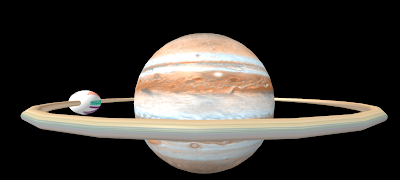
\includegraphics[width=10cm]{chapters/chapter2/figures/Picture1.png}
    \caption{Starting point}
    \label{fig:Picture1}
\end{figure}


\section{It needs a moon}
The process is really just combining elements of the steps 1-3. Create a new sphere,set the radius to something around 0.25 to 0.5; colour it with whatever you feel is appropriate, add an image (in the example code one has been added) if you want, set a rotation (it is is fun to play with these a bit and place the moon on the ring (setting position="5 0 0" in this case does this.

If the images are accessible as web sources this could be a great option.

Lets put a moon on the ring between
\begin{lstlisting}
<a-torus>
\end{lstlisting} 
\begin{lstlisting}
</a-torus>
\end{lstlisting} 


So the code for the moon
\begin{lstlisting}
    <a-sphere position="5 0 0"
        rotation="0 0 0"
        radius="0.5"
        color="yellow" src="https://cdn.glitch.com/febf6408-3c33-4608-
        ac90-b087753e5792%2Fpanic.png?v=1573395380360"
        animation="property: rotation; 
        to:  0 259 0; loop: true; dur: 3000">
    </a-sphere>
\end{lstlisting}
Gets put inside that of the torus, so the whole thing becomes
\begin{lstlisting}
<html>
  <head>
    <script src="https://aframe.io/releases/0.9.2/aframe.min.js">
    </script>
  </head>
  <body>
    <a-scene>
     <a-sphere position="0 1.25 -5" radius="3" 
     color="white" src="https://cdn.glitch.com/febf6408-3c33-4608-ac90-b0877
     53e5792%2F2k_jupiter.jpg?v=1573393224376"
    animation="property: rotation; to: 0 360 0; loop: true; dur: 10000">
        <a-torus position="0 0 0" arc="360"
                rotation="90 0 0"
                color="white" radius="5"
                radius-tubular="0.05"
                animation="property: 
                rotation; to:  90 90 0; 
                loop: true; dur: 3000">
                <a-sphere position="5 0 0"
                 rotation="0 0 0"
                 radius="0.5"
                 color="yellow" src="https://cdn.glitch.com/febf6408-3c33-460
                8-ac90-b087753e5792%2Fpanic.png?v=1573395380360"
                 animation="property: 
                 rotation; to:  0 259 0; 
                 loop: true; dur: 3000">
              </a-sphere>
         </a-torus>
      </a-sphere>   
      <a-sky color="black"></a-sky>
    </a-scene>
  </body>
</html>               
\end{lstlisting}

\section{Let's add text and stars}
So we might want to put some text into the world we can do that with
\begin{lstlisting}
<a-text value=””>
\end{lstlisting} 

So adding this to the code (see below) put a message on the screen, though you may have to use the down arrow to see it.

\begin{lstlisting} 
<html>
  <head>
    <script src="https://aframe.io/releases/0.9.2/aframe.min.js">
    </script>
  </head>
  <body>
    <a-scene>
     <a-sphere position="0 1.25 -5" radius="3" 
     color="white" src="https://cdn.glitch.com/febf6408-3c33-4608-ac90-b087753e5792%2F2k_jupiter.jpg?v=1573393224376"
               animation="property: 
               rotation; to: 0 360 0; loop: true; 
               dur: 10000">
        <a-torus position="0 0 0" arc="360"
            rotation="90 0 0"
            color="white" radius="5"
            radius-tubular="0.05"
            animation="property: rotation; 
            to:  90 90 0; loop: true; dur: 3000">
                <a-sphere position="5 0 0"
                 rotation="0 0 0"
                 radius="0.5"
                 color="yellow"
             src="https://cdn.glitch.com/febf6408-3c33-4608
             -ac90-b087753e5792%2Fpanic.png?v=1573395380360"
                 animation="property: rotation; 
                 to:  0 259 0; 
                 loop: true; dur: 3000">
              </a-sphere>
         </a-torus>
      </a-sphere>   
      <a-text value="Planet CCCU Computing" 
      position="0 4 -2">
      </a-text>
      <a-sky color="black"></a-sky>
    </a-scene>
  </body>
</html>
\end{lstlisting}

\begin{figure}
    \centering
    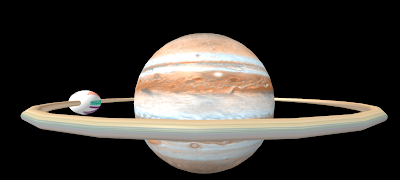
\includegraphics[width=10cm]{chapters/chapter2/figures/Picture1.png}
    \caption{Starting point}
    \label{fig:Planet again}
\end{figure}

We can get interesting effects if we add the text between \begin{lstlisting}
</a-sphere>
\end{lstlisting}
\begin{lstlisting}
</a-torus>
\end{lstlisting}  

Try adding this in there. \begin{lstlisting}
<a-text value="Planet CCCU Computing" position="0 3 -2"></a-text>
\end{lstlisting}

Have a play with altering the text and putting the line elsewhere in the code. What happens?

Now going to use an image to change the background. The image is "space" by fleskw is licensed with CC BY 2.0. To view a copy of this license, visit \url{https://creativecommons.org/licenses/by/2.0} You will need to change the sky colour to a light colour for this to work. 

So change the sky line in the code to white we are going to use the space image to make it a bit easier it is in this form \url{https://cdn.glitch.com/425c1a98-7ba9-463d-817d-6b491a516246%2F97b3bf6d-ced1-4041-80d4-b6c9a98ba43d.jfif?v=1614341330757} 

\begin{lstlisting}
<a-sky color="white" src="https://cdn.glitch.com/425c1a98-7ba9
-463d-817d-6b491a516246%2F97b3bf6d-ced1-4041-
80d4-b6c9a98ba43d.jfif?v=1614341330757">
</a-sky>
\end{lstlisting}
Now adding it the code in place of the current 
\begin{lstlisting}
<a-sky>\end{lstlisting}

We get.
\begin{lstlisting}
<html>
  <head>
    <script src="https://aframe.io/releases/0.9.2/aframe.min.js">
    </script>
  </head>
  <body>
    <a-scene>
     <a-sphere position="0 1.25 -5" radius="3" 
     color="white" src="https://cdn.glitch.com/
     febf6408-3c33-4608-ac90-b087753e5792%2F2k_jupiter.jpg?v=1573393224376"
               animation="property: rotation; 
               to: 0 360 0; 
               loop: true; dur: 10000">
        <a-torus position="0 0 0" arc="360"
                rotation="90 0 0"
                color="white" radius="5"
                radius-tubular="0.05"
                animation="property: rotation; 
                to:  90 90 0; loop: true; dur: 3000">
                <a-sphere position="5 0 0"
                 rotation="0 0 0"
                 radius="0.5"
                 color="yellow" src="https://cdn.glitch.com/febf6408-3c33-4608-ac90-b087753
                 e5792%2Fpanic.png?v=1573395380360"
                 animation="property: rotation; to:  0 259 0; 
                 loop: true; dur: 3000">
              </a-sphere>
         </a-torus>
      </a-sphere>   
      <a-text value="Planet CCCU Computing" position="0 4 -2"></a-text>
      <a-sky color="white" src="https://cdn.glitch.com/425c1a98
      -7ba9-463d-817d-6b491a516246%2F97b3bf6d-ced1-4041-80d4-
      b6c9a98ba43d.jfif?v=1614341330757">
      </a-sky>
    </a-scene>
  </body>
</html>
\end{lstlisting}

We are done!

\begin{figure}
    \centering
    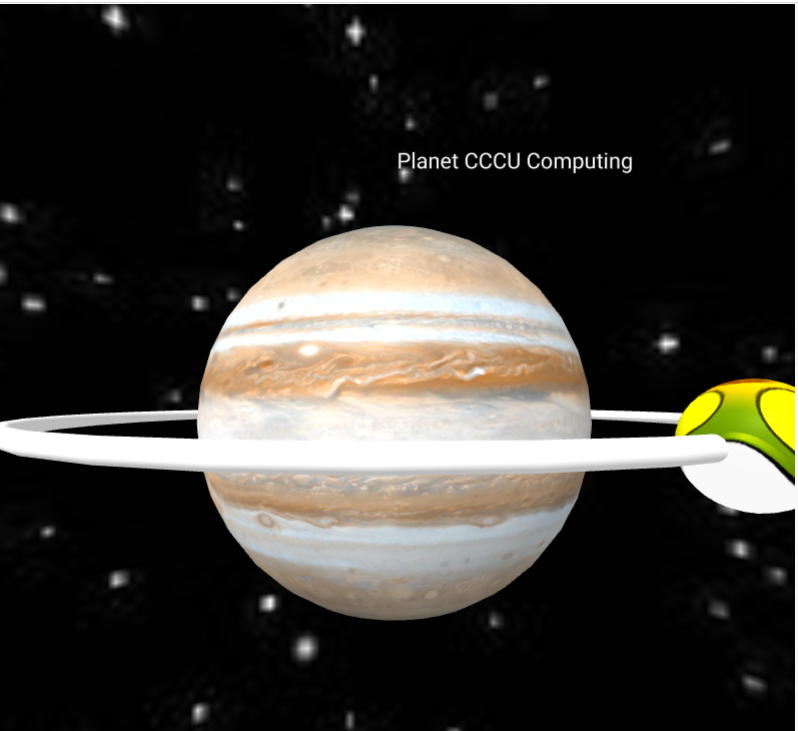
\includegraphics[width=10cm]{chapters/chapter2/figures/planet3.png}
    \caption{Starting point}
    \label{fig:Planet3}
\end{figure}
\chapter{Augmented Reality : Markerbased and location-based}

\section{Introduction}
For a few years, I have been a fan of Aframe and AR.js - these are fantastic tools for creating web-based Virtual and Augmented Reality.

\section{Marker-based}
Now AR.js has just got easier - no coding need with the Beta version of AR.js Studio \url{https://ar-js-org.github.io/studio/}

\begin{figure}
    \centering
    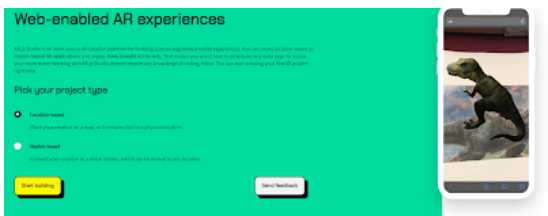
\includegraphics[width=10cm]{chapters/ChapterAR/webar1.png}
    \caption{AR.JS studio}
    \label{fig:arjsstudio}
\end{figure}

I am going to use the premade marker but you can upload your own, there is a guide to what makes a good marker. The premade marker you can download from the site using the download marker link underneath the marker. Apart from that, you don't have to do anything else to select the marker
\begin{figure}
    \centering
    
\includegraphics[width=5cm]{chapters/ChapterAR/webar6.png}
    \caption{marker}
    \label{fig:marker}
\end{figure}

Now you choose whether you want 3D object, image or video. So for this experiment, I going to use a free 3D model from \url{https://sketchfab.com/3d-models/duck-6e039c6c606c4c26a1359514352629fd} produced by likangning93 and released under a creative commons licence on Sketchfab. It is as simple as clicking upload file and browsing.

\begin{figure}
    \centering
    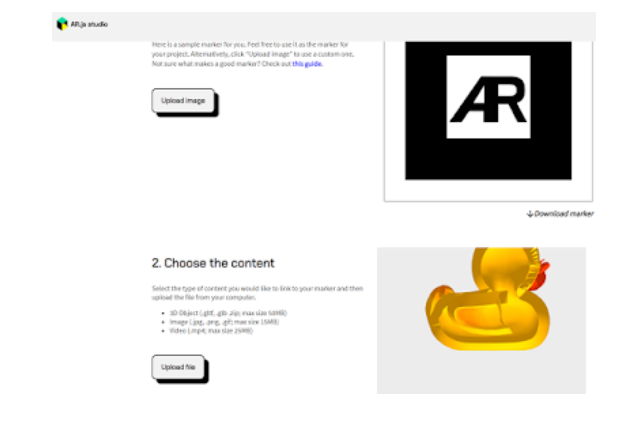
\includegraphics{chapters/ChapterAR/webar5.png}
    \caption{set up}
    \label{fig:my_setup}
\end{figure}

Last stage is exporting the project. Two options 
- Published to Github 
- Download package

My advice is, if you don't have your own web-server, get yourself a Github account and choose that option, and you just log-in to your account. You will need to give the project a name and then push Publish. Depending on your internet connection it can take a few seconds to a minute or so, but it is worth the wait.

So now you get back a \url{https://scottturneruon.github.io/Testobjectexs5y2/} 

Now just show the marker.
\begin{figure}
    \centering
    
\includegraphics[width=5cm]{chapters/ChapterAR/webar6.png}
    \caption{marker}
    \label{fig:marker}
\end{figure}

So to test I am typing this URL in a Safari browser (Chrome can play up) on my phone and allow access to my camera (see below or try it for yourself which is more fun).

\begin{figure}
    \centering
    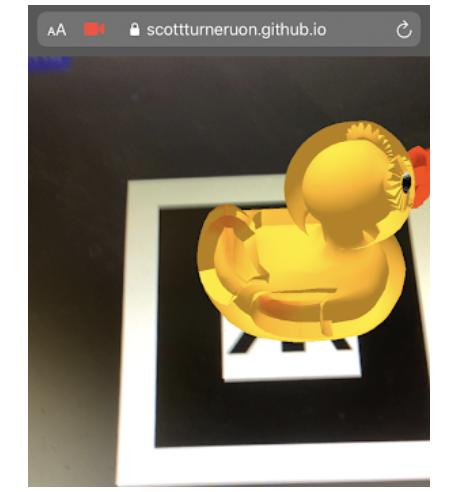
\includegraphics{chapters/ChapterAR/webar7.png}
    \caption{Floating duck}
    \label{fig:floatingduck}
\end{figure}

This Beta version is very good, no coding needed by the user and easy steps to an AR.  At the time of writing the only slight issue was you need to ensure that the file extensions were not capitalised but other than it is a great tool for produce a single AR example. I need to try the location-based version next.



\section{Location-based}
 Now AR.js has just got easier - no coding need with the Beta version of AR.js Studio  including using markers and the focus of this post, geo-located or markerless AR.
 
 It so easy I am going to show two examples. First going to the start screen of AR.js Studio https://ar-js-org.github.io/studio, select location based project type.
 
\begin{figure}
    \centering
    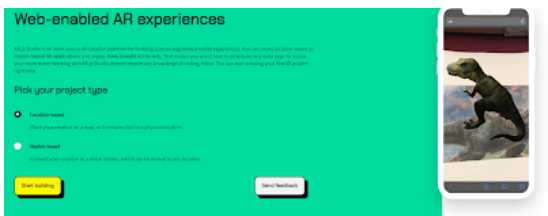
\includegraphics[width=10cm]{chapters/ChapterAR/webar1.png}
    \caption{AR.JS studio}
    \label{fig:arjsstudio}
\end{figure}
 
 You will then be asked for the longitude and latitude on where you want your AR to be located, up to 10 locations can be used - I have only used one to trial it. If you don't know these co-ordinates they have included a link to a site \url{https://www.latlong.net/}  that will give you these and you can then transfer them into AR.js Studio that is the geo-location bit done. Now for the thing at the location.
 
 
So for the first experiment, I going to use a free 3D model from \url{https://sketchfab.com/3d-models/duck-6e039c6c606c4c26a1359514352629fd}  produced by likangning93 and released under a creative commons licence on Sketchfab. It is as simple as clicking upload file and browsing. The last stage is publishing it on GitHub and you getting a URL or downloading the files and which you can later add to a server - both really just a click option. 

So the Duck is shown below 

\begin{figure}
    \centering
    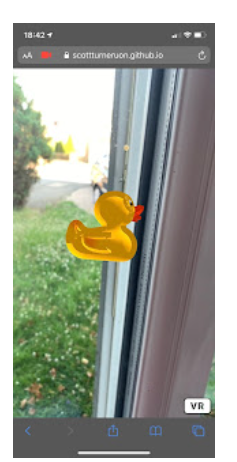
\includegraphics[width=10cm]{chapters/ChapterAR/webar3.png}
    \caption{Marker-less Duck}
    \label{fig:markerless_duck}
\end{figure}

So as a follow up and as I think Jupiter is such as a beautiful planet, I used a model by Miekle Roth on Sketchfab \url{https://sketchfab.com/3d-models/jupiter-c5275eb96af245e4a8453837ac728a62}  as a second geolocated object. 

So now I have Jupiter whenever I want - no I am not that power-mad.
 \begin{figure}
     \centering
     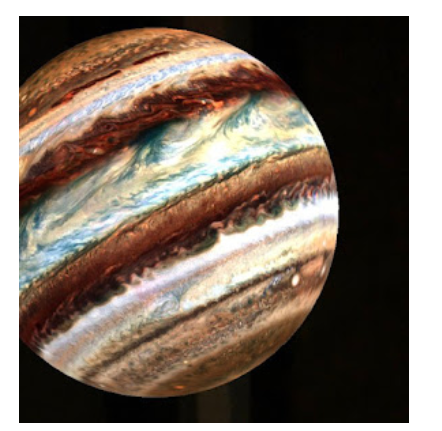
\includegraphics{chapters/ChapterAR/webar4.png}
     \caption{Jupiter}
     \label{fig:jupiter}
 \end{figure}
 
 Some interesting things I noticed it is relatively easy to do it, and I think the resources downloaded through AR.js Studio could be a great start on a more complex project. Initially, I didn't have location turned on my phone (obvious I know) but I could still see the object when I looked down - so that is great feature to have when you are trying out markerless AR to see what it could look like. 

Try AR.js Studio \url{https://ar-js-org.github.io/studio} for yourself.

\part{Physical Computing}
\chapter{EGGbot}
\section{inspiration}
Three inspirations for this project
·      Eggbot - \url{http://www.instructables.com/id/Plastic-Egg-Bot/}
 
·  	Femi Owolade supported by Nic Hughes ran a session at Mozilla Festival 2016 using the Crumble’s to make a wheeled robot.
 
·  	The junkbot project \url{https://junkbots.blogspot.co.uk/}

\section{Kit}
\begin{itemize}
    \item Kinder Egg (without the Chocolate and toy)
    \item Crumble Controller available at \url{https://redfernelectronics.co.uk/shop/}
    \item 4x Crocodile clips and leads
    \item Battery pack and 3xAA batteris
    \item Vibrating motor or small DC motor with a weight added to the axel
    \item Tape (lots of)
    \item Pens
    \item Paper
    \item Scissors
    \item Glue and Gluegun (optional)
\end{itemize}
\section{Stage1: Fix the vibrating motor into the Egg.}

Put the vibrating motor into the Egg with the motor electrical connections sticking out the bottom larger half of the egg. Make sure the unbalanced load is free to move – this is bit that causes the vibrations needed to move the egg. The motor can be held in place by sticky-tack or strong tape, or glue (when using glue this is done under adult supervision only)

\begin{figure}
    \centering
    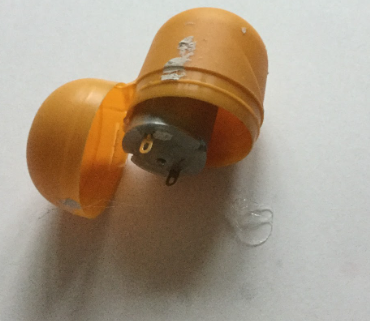
\includegraphics[width=10cm]{chapters/ChapterP1/figures/eggbot_stage1.png}
    \caption{Eggbot drawing stage 1}
    \label{fig:Egggbotdrawing1}
\end{figure}

\section{Stage 2: Sticking the pens on}

This is the trickiest bit. The easiest way to do is cut a strip of tape. Place two pens onto the tape ensuring the pens are the same length from the tape to the nib and the distance between the pens on the tape are far enough apart to place the egg between them.

\begin{figure}
    \centering
    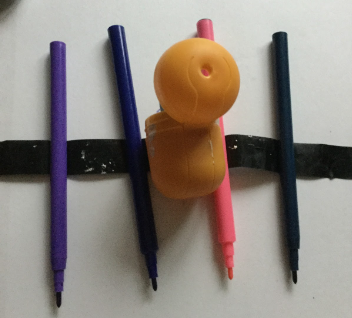
\includegraphics[width=10cm]{chapters/ChapterP1/figures/eggbot_stage2.png}
    \caption{Eggbot drawing stage2}
    \label{fig:Egggbotdrawing2}
\end{figure}

If you are using three pens, the third pen should be placed so that all three form a triangle with equal sides, that means the egg can stand-up on a piece of paper on the pen nibs, without anything supporting it.
 
If you are using four pens, the other two pens should be placed so that all four form a square with equal sides, that means the egg can stand-up on a piece of paper on the pen nibs, without anything supporting it.

\section{Stage 3: Add the battery pack and go.}

Using two wires connecting the battery, to the motors. Remove the nibs and set the bot off. It is hopefully vibrating and shaking and scribbling lines on the paper.

\begin{figure}
    \centering
    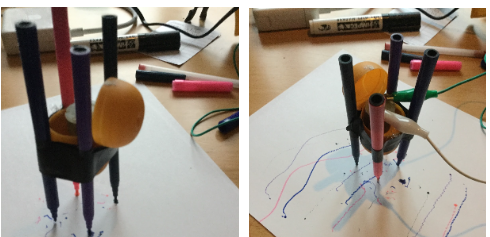
\includegraphics[width=10cm]{chapters/ChapterP1/figures/eggbot_stage3.png}
    \caption{Eggbot drawing stage3}
    \label{fig:Egggbotdrawing3}
\end{figure}


To see one in action go to: 
\url{https://www.youtube.com/watch?v=NRlntdmdQRo}

\section{Stage 3: Add Control (sort of) Crumble}

Disconnect the battery connection (the connections on the motor can stay as they are). Connect the USB cable to the Crumble. To the right of the USB connect there are two connections marked + and -. Connect a Red wire to the + connection and the other end to the red wire of the battery pack. Connect a black wire to the – connection and the other end to the black wire of the battery pack.

\begin{figure}
    \centering
    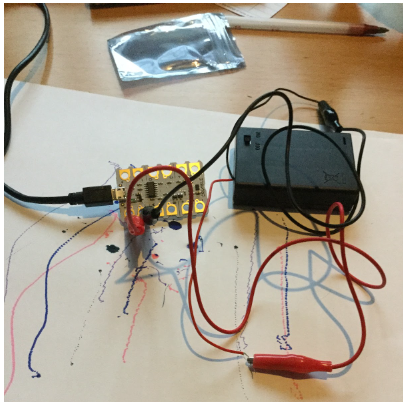
\includegraphics[width=10cm]{chapters/ChapterP1/figures/eggbot_stage4.png}
    \caption{Eggbot drawing with crumble}
    \label{fig:EgggbotdrawingCrumble}
\end{figure}

On the Crumble, on the right-side there are two motor connections connect the Motor to these connections. Don’t worry about which of the motors wires is need you swap them around later.

\begin{figure}
    \centering
    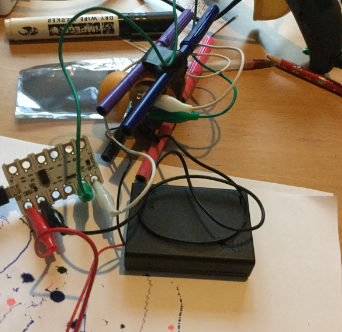
\includegraphics[width=10cm]{chapters/ChapterP1/figures/eggbot_stage5.png}
    \caption{Eggbot and crumble}
    \label{fig:EgggbotdrawingCrumble2}
\end{figure}

\section{Stage 4: ALet's start programming it}

The software can be found at \url{https://redfernelectronics.co.uk/crumble-software/} it includes how to set it up on your own machine.
 
Start the Crumble software. Drag from the left the Program start, motor, and wait blocks. Now join the up start block at the top and the motor block next and the wait block last.


\begin{figure}
    \centering
    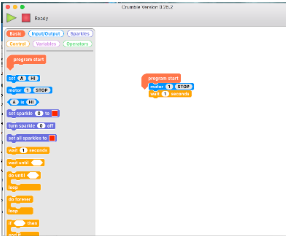
\includegraphics[width=10cm]{chapters/ChapterP1/figures/eggbot_stage6.png}
    \caption{Eggbot and crumble code}
    \label{fig:EgggbotdrawingCrumble3}
\end{figure}

Your code should look like this.

\begin{figure}
    \centering
    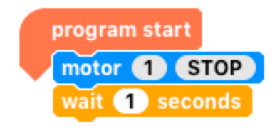
\includegraphics[width=10cm]{chapters/ChapterP1/figures/eggbot_stage7.png}
    \caption{Eggbot and crumble code initial}
    \label{fig:EgggbotdrawingCrumble4}
\end{figure}

Click on the stop within the motor block. It should change to forward. Now you are ready to make it move. Press the green arrow and with the battery pack on, it should (hopefully) keep moving.

\begin{figure}
    \centering
    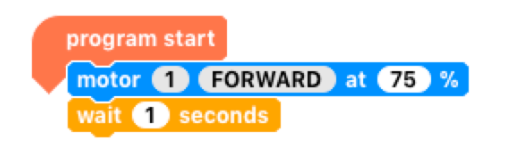
\includegraphics[width=10cm]{chapters/ChapterP1/figures/eggbot_stage8.png}
    \caption{Eggbot and crumble - start}
    \label{fig:EgggbotdrawingCrumble5}
\end{figure}

If you put a second motor block after the wait block with the stop in the block. It such then stop after 1 second of moving.

\section{Stage 5: Making it do more}
.
-   	Drag a do-until block in (found in the control menu).
-   	Go to variable menu and add a new variable, I have used t, select the block marked let=, and drag a t into the blank space.
-   	Drag an increase block onto the screen and drag a t into the blank space.


\begin{figure}
    \centering
    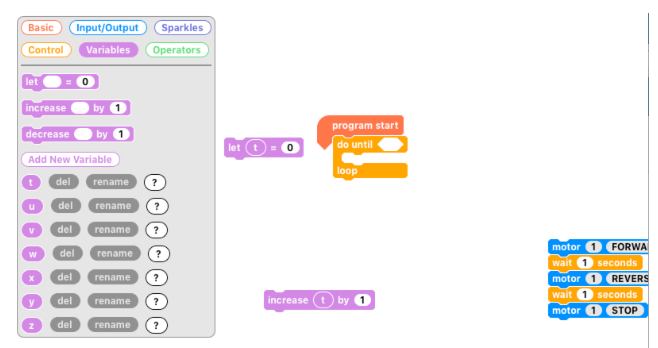
\includegraphics[width=10cm]{chapters/ChapterP1/figures/eggbot_stage9.png}
    \caption{Eggbot and crumble - Lets do a little more}
    \label{fig:EgggbotdrawingCrumbleMore1}
\end{figure}

Go to the operator menu and drag onto the screen an = block, go back to variables menu and drag a t into the first space on the = block and click on the second space on the block and type in 5.

\begin{figure}
    \centering
    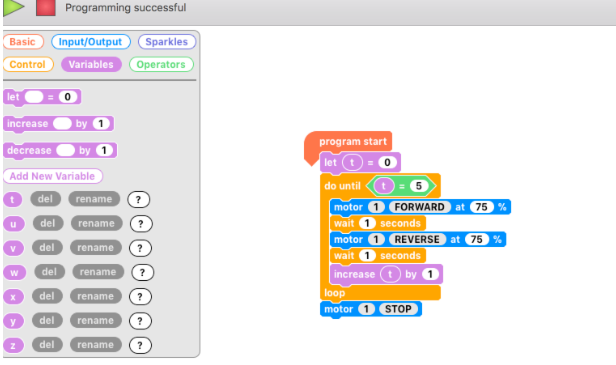
\includegraphics[width=10cm]{chapters/ChapterP1/figures/eggbot_stage10.png}
    \caption{Eggbot and crumble - Lets take it a  little further}
    \label{fig:EgggbotdrawingCrumbleMore2}
\end{figure}

Now for the challenge put all these together to copy what is shown below. Now, put the egg-bot on the paper, with the pen lids off, press the green triangle and the motors should be spun in different directions.
 
This is a junkbot so it may just cause the bot to move a slightly different directions but hopefully it should just draw some squiggly lines.
\chapter{Microbit V1 data logging}
\section{Why?}
Often we need applications that allow collection of data over time, for example temperature or light levels through the day. Allowing us potentially analyse the data for trends. The microbit is a fantastic tool with some of these sensors already in place (e.g. light and temperature) or can be added to with extra sensors from add-on boards (such as Kitronik Air Quality and Environmental Board for micro:bit https://shop.pimoroni.com/products/kitronik-air-quality-and-environmental-board-for-micro-bit?variant=39475687227475 )

Datalogging with a V2 microbit is relatively easy all the details are available here: https://microbit.org/get-started/user-guide/data-logging/ to get started. 

But what about the older V1 can it do it?

The answer is yes but it is a little more work and is generally a little more limited but still very worth while. In this article we are going to look at doing this.
spot.co.uk/}

\part{Computational Thinking}

\chapter{Thomas's Tangles}
A recently released book Teaching Computing Unplugged in Primary Schools  edited by Helen Caldwell (University of Northampton) and Neil Smith (Open University) has a number of interesting chapters by authors who are passionate about how computing is taught in schools. The central theme is unplugged activities, without using computers, but still teach the fundamental of computational thinking.

Ok, confession time. I co-wrote, along with Katharine Childs (Raspberry Pi Foudation), Chapter 3 Artists so I am biased here, but I believe in the central theme of Unplugged Computing. Computing, and Computational Thinking in general,  is not just about programming and using a computer (though using computers and  programming are vitally important to Computing) but it is also about many other things including problem-solving, being creative and working collaboratively.

Chapter 3 is about linking these computational thinking ideas to produce visual art, by applying computing principles including  repetition, following and refining algorithms, and abstraction. The chapter also looks, how these links have already being made, with examples such Sol Le Witt where not all the work that was produced by the artist himself, but some by others following his written instructions - in other words an algorithm. There is even a game Thomas's Tangles

The other chapters make links with areas such as Robots, Musicians, Explorers, Magicians, Gamers, Cooks and Scientists.

\section{Thomas Tangles}
This simplifies the algorithm Thomas' Tangles (named after my son who helped develop it) in Chapter 3 of the book discussed in http://compuationalthinking.blogspot.co.uk/2016/11/how-to-be-unplugged-artist.html

Using crayons, pencils or pens, we are going to follow an algorithm to create a random drawing. This could be done in pairs and you will need squared paper. 

Person A: Rolls the dice and reads out the instructions - their role is to roll the dice, interpret the algorithm and tell the 'robot' what to do.

Person B: Is the ‘robot carrying out the instructions'. The lines are solid blocks of colour so move four squares does also mean colour in the squares between the start and finish in the direction of movement.

\begin{figure}
    \centering
    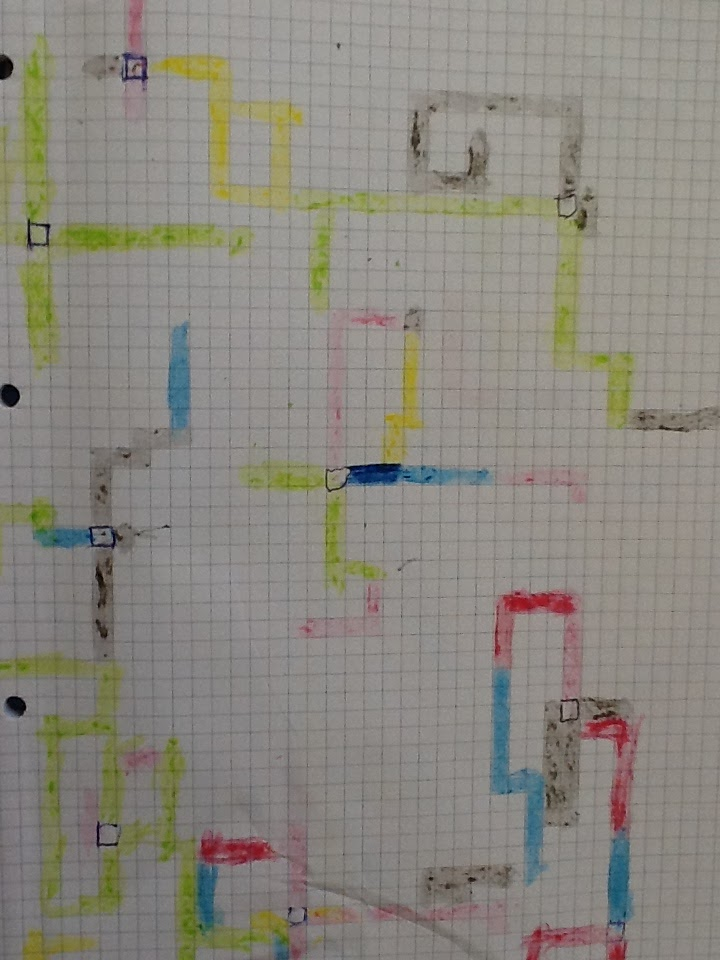
\includegraphics[width=10cm]{chapters/chapterCT1/figures/tt1.JPG}
    \caption{Thomas' Tangles}
    \label{fig:ThomasTangles1}
\end{figure}

When a new central square is needed the roles of A and B swap (so A is the ‘robot’ and B rolls the dice and reads out the instruction). The roles keep swapping.

\begin{lstlisting}
Start from a random square – call it the centre square
Repeat until end of game
If die roll = 1
  Roll die for number of moves
 move die roll number of steps up the page
If die roll = 2
  Roll die for number of moves
  move die roll number of steps down the page
If die roll = 3
  Roll die for number of moves
  move die roll number of steps to the left 
If die roll = 4
  Roll die for number of moves
  move die roll number of steps to the right
If die roll = 5
  Roll die
  If die = 1 change colour to Red
  If die = 2 change colour to Blue
      If die = 3 change colour to Black
  If die = 4 change colour to Green
  If die = 5 change colour to Orange
  If die = 6 change colour to Yellow
If die roll = 6
           Roll die
  Return to current centre square
                If the second die roll=6
                   randomly select new centre square
     if block is off the page
                randomly select new centre square
\end{lstlisting}

The Scratch version can be here \url{https://scratch.mit.edu/projects/135816631/} if you wish to see the code.


\chapter{Music}
\section{Scratch}


\section{Sonic Pi}


The goal - spooky/moanful Hot-Cross Buns (the only bit of music I know the notes for), just so I can play a bit. So let us start with resources I have found useful, alongside Sonic Pi (https://sonic-pi.net/; a really useful webpage is \url{https://newt.phys.unsw.edu.au/jw/notes.html}  to turn the notes into the MIDI number (60, etc) 

So by the end of the last post I got to adding a techno effect on top of the tune:
\begin{lstlisting}
use_synth :prophet
with_fx :ixi_techno do
  2.times do
    play chord(:b4, :minor7)
    sleep 0.5
    play chord(:a4, :minor7)
    sleep 0.5
    play chord(:g4, :minor7)
    sleep 0.5
  end
  4.times do
    play chord(:g4, :minor7)
    sleep 0.25
  end
  4.times do
    play chord(:a4, :minor7)
    sleep 0.25
  end
  play chord(:b4, :minor7)
  sleep 0.5
  play chord(:a4, :minor7)
  sleep 0.5
  play chord(:g4, :minor7)
  sleep 0.5
end
\end{lstlisting}


Sonic Pi is a cool system I found out you get it to pan the sounds from left to right and played with that but didn't include it in the end. What I did change in was a different synth but also samples, after trail-and-error, chose the ambi_dark_whoosh (had to with that name)
\begin{lstlisting}
use_synth :tech_saws
sample :ambi_dark_woosh, amp: 0.25
with_fx :ixi_techno do
  2.times do
    play chord(:b3, :minor7)
    sleep 0.5
    play chord(:a3, :minor7)
    sleep 0.5
    play chord(:g3, :minor7)
    sleep 0.5
  end
  sample :ambi_dark_woosh, amp: 0.25
  4.times do
    play chord(:g3, :minor7)
    sleep 0.25
  end
  4.times do
    play chord(:a3, :minor7)
    sleep 0.25
  end
  sample :ambi_dark_woosh, amp: 0.25
  play chord(:b3, :minor7)
  sleep 0.5
  play chord(:a3, :minor7)
  sleep 0.5
  play chord(:g3, :minor7)
  sleep 0.5
end
\end{lstlisting}



This is a bit of software (and support on Patreon) it is just fun and free. I have no musical ability but I enjoy creating with it.
\chapter{Magic}
\section{Inroduction}
\section{Which one did you change?}
So we are going to produce a 8x8 grid of elements that we can change to one of two states. It could be a grid of 64 post-it notes of two colours or dots on the screen.
\begin{figure}
    \centering
    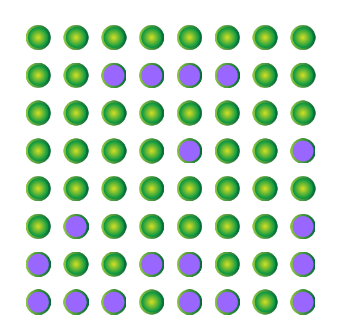
\includegraphics[width=3cm]{chapters/chapterCT1/figures/paritygame.png}
    \caption{Parity Game}
    \label{fig:Parity Game in Scratch}
\end{figure}
\newline
The Scratch code for this can be found at \url{https://scratch.mit.edu/projects/742512502/}
\newline
Now for the first seven rows and first (starting from the left) elements of the grid set the elements to one of the two possible states/colours. 
\begin{figure}
    \centering
    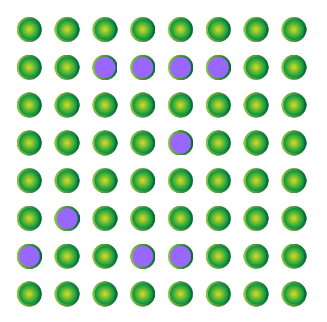
\includegraphics[width=3cm]{chapters/chapterCT1/figures/paritygame2.png}
    \caption{Parity Game starting point}
    \label{fig:Parity Game starting point}
\end{figure}
\newline
So for each row make the number of a particular state be even, so as an example on the fourth row from the top there is only 1 purple dot, so in the last dot on the row we change it from green to purple so there are even number of purple dots on that row. We repeat this for each of the first seven rows. We then do the same for the columns making all the dots in the column be an even number (including the last column) by including a purple dot or not as appropriate.

Now for the trick. Get someone to change one of the dots while the magician looks away. When the magician comes back they are looking for the row and column where the number of particular coloured dot are odd numbered this tells you on which row and column the dot was changed,

This is a concept called Parity where we by making sure all rows and columns have even numbers of particular coloured dots (and you could equally do this with making sure all are odd numbers of particular dots) by adding dots into the extra column and row, we can have built a check for a change.

In Computing we can use this idea to check for an error. Instead of dots, imagine we have 1 or 0 (binary) if we want to transmit 7 bits and we use the 8th bit to make sure the numbers of 1 bits is even when we send the signal (7 bits and the extra bit), if a bit has changed when we recieve it has an odd number of bits, an error has been detected. If we sent the data as 8 blocks with the last 'row' been made up of the bits that make the columns have even number of ones then this will also have change if a single bit has changed but only in the row and column that the changed/error occured so we find the bit and change it back - error correction.

\section{What day of the month is your birthday?}
It is simple but this 'trick' shows the principles of binary and the power of algorithms.I wish I had invented this one.

1.	Say to the participant "If you answer 5 simple questions I can predict which number in the month your birthday is on"

2.	Question 1 "Is the number in Box A?" If the number is the box add 1 otherwise don't add anything. The Magician keeps a running total of the scores.
\newline
\begin{figure}
    \centering
    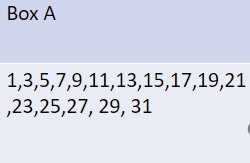
\includegraphics[width=3cm]{chapters/chapterCT1/boxA.png}
    \caption{Box A}
    \label{fig:Box A}
\end{figure}
\newline
3.	Question 2 “Is the number in Box B?" If the number is the box add 2 otherwise don't add anything
\newline
\begin{figure}
    \centering
    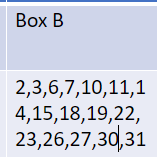
\includegraphics[width=3cm]{chapters/chapterCT1/BoxB.png}
    \caption{Box B}
    \label{fig:Box B}
\end{figure}
\newline
4.	Question 3 “Is the number in Box C?" If the number is the box add 4 otherwise don't add anything
\begin{figure}
    \centering
    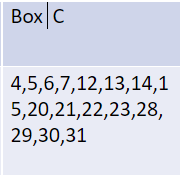
\includegraphics[width=3cm]{chapters/chapterCT1/BoxC.png}
    \caption{Box C}
    \label{fig:Box C}
\end{figure}
5.	Question 4 “Is the number in Box D?" If the number is the box add 8 otherwise don't add anything.
\begin{figure}
    \centering
    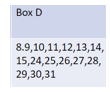
\includegraphics[width=3cm]{chapters/chapterCT1/figures/boxD.png}
    \caption{Box D}
    \label{fig:Box D}
\end{figure}
6.	Question 5 “Is the number in Box E?" If the number is the box add 16 otherwise don't add anything.
\begin{figure}
    \centering
    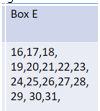
\includegraphics[width=3cm]{chapters/chapterCT1/figures/BoxE.png}
    \caption{Box E}
    \label{fig:Box E}
\end{figure}
7.	Your running total should be the number
What have you done: You have used binary to find the number. For example 27 would be in Box E, Box D , Box B and Box A.which in if we replace the boxes with 1 if the number is in there and 0 if it isn’t; when the boxes are ordered E D C B A we get 11011 which is 27 in decimals. We also have used an algorithm instructions 1 to 6 to get there.
\newline
So lets make it a bit more 'Computer Sciencey,'
Now if we place them into a Table 
\begin{tabular}{lllll} \hline
E & D & C & B & A	 	 \\ \hline
1  & 1  & 0 &  1 & 1\\ \hline

\end{tabular}

Lets instead of A to E we replace the labels with 1, 2,4. 8, 16 each one is the double of the earlier we get:


So 27 is 11011 in binary
\begin{tabular}{lllll} \hline
32 & 16 & 8 & 2 & 1 	 \\ \hline
1  & 1  & 0 &  1 & 1\\ \hline

\end{tabular}

\section{Sorting out VIPS}
\chapter{Translation in Scratch}

\section{Text to speech and translate}
Scratch 3 the gift that keeps on giving; including the new extensions are Text to Speech and Translate; Text to speech - does as the name suggests, turns typed in phrases into speech via Amazon Web Services. Translate using Google (and I assume Google Translate?) to translate text between different languages.

\begin{figure}
    \centering
    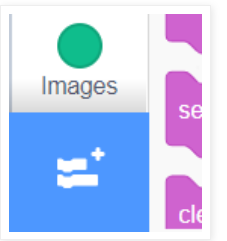
\includegraphics[width=5cm]{chapters/chapterCT1/figures/translat1.png}
    \caption{Extensions button}
    \label{fig:Scratch_extension_button}
\end{figure}

\begin{figure}
    \centering
    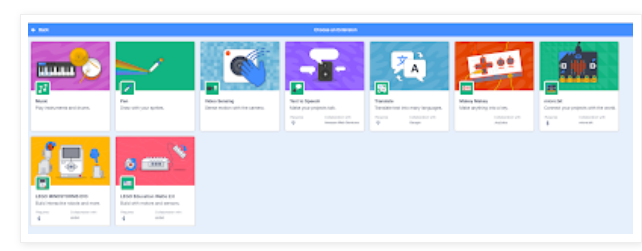
\includegraphics[width=7cm]{chapters/chapterCT1/figures/translate7.png}
    \caption{Scratch_extensions}
    \label{fig:mextensions_l}
\end{figure}


As an experiment, I wanted to  have Scratch the Cat ask me to enter a phrase and then convert that into French, German and Spanish with different voices. The resulting code is shown below.

\begin{figure}
    \centering
    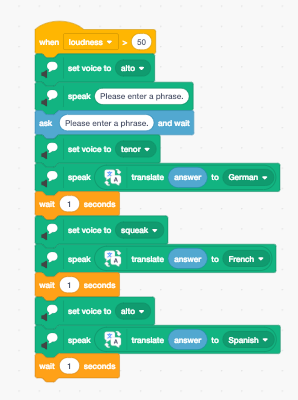
\includegraphics{chapters/chapterCT1/figures/translate8.png}
    \caption{Scratch code to translate}
    \label{fig:scratch_trnslate}
\end{figure}


It is all started by a loud noise like a hand clap. The two extensions have been added to the blocks and are ready to go. The voice is initially set to Alto and the text-speech block has had the phrase "Please enter a phrase" typed in and says this. The ask block has the same question permanently set and the answer produced gets feed into the translations. 

The remaining blocks do essentially the same thing
- change the voice;
- take the phrase typed in (via answer) and convert to the language of choice;
- wait a second.


It is great fun, I am not sure all the languages work but what is there is cool to play with. In an ideal world instead of typing the phrase it would be great to just say the phrase...maybe in the future. 

The code is available at https://scratch.mit.edu/projects/282312832/.
originally published in \url{https://robotsandphysicalcomputing.blogspot.com/2019/01/scratch-speaking-german-french-spanish.html}

\section{speech recognition}
originally published in \url{https://robotsandphysicalcomputing.blogspot.com/2020/07/speech-recognition-turning-hello-into.html}

The Raspberry Pi Foundation recently released a programming activity Alien Language, with support Dale from Machine Learning for Kids, that is a brilliant use of Scratch 3 - Speech Recognition to control a sprite in an alien language. Do the activity, and it is very much worth doing, and it will make sense! I  would also recommend going to the machinelearningforkids.co.uk site anyway it is full of exciting things to do (for example loads of activities https://machinelearningforkids.co.uk/#!/worksheets ). Scratch 3 has lots of extensions that are accessible through the Extension button in the Scratch 3 editor (see below) which add new fun new blocks to play with.




The critical thing for this post is Machine Learning for Kids have created a Scratch 3 template with their own extensions for Scratch 3 within it https://machinelearningforkids.co.uk/scratch3/. One of which is a Speech to Text extension (see below). You must use this one not the standard Scratch 3.

\begin{figure}
    \centering
    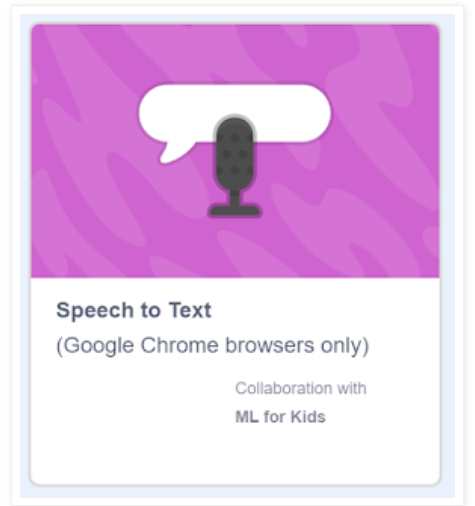
\includegraphics[width=7cm]{chapters/chapterCT1/figures/translate2.png}
    \caption{Speech to Text extension}
    \label{fig:speech to text}
\end{figure}


My idea is to can I set it to react one way when I say "hello"; then say "french" and then say "hello" it says "Bonjour". Two other extensions are needed along with the Speech to Text one - one for speech to text and the translate shown below.

\begin{figure}
    \centering
    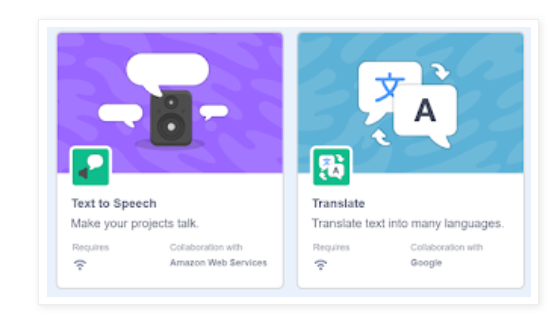
\includegraphics[width=7cm]{chapters/chapterCT1/figures/translate3.png}
    \caption{Other extensions}
    \label{fig:other_extensions}
\end{figure}


Ok, so to the fun bit. The listen and wait, and when I hear blocks are the key new blocks, and they do what they say. The three sets of the code are ones I used for this activity.

\begin{figure}
    \centering
    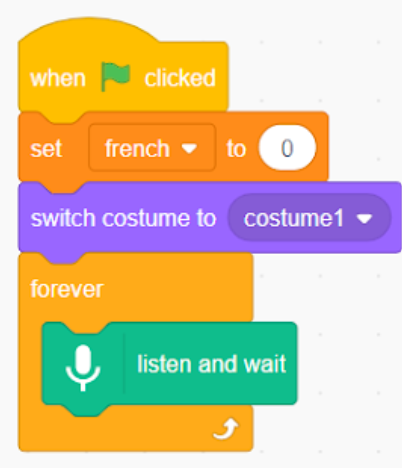
\includegraphics[width=6cm]{chapters/chapterCT1/figures/translate4.png}
    \caption{code 1}
    \label{fig:code1}
\end{figure}
\begin{figure}
    \centering
    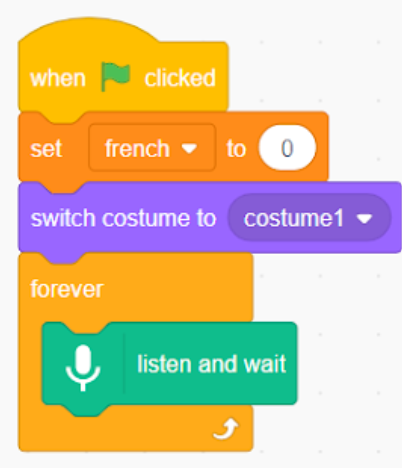
\includegraphics[width=6cm]{chapters/chapterCT1/figures/translate5.png}
    \caption{Code2}
    \label{fig:code2}
\end{figure}
\begin{figure}
    \centering
    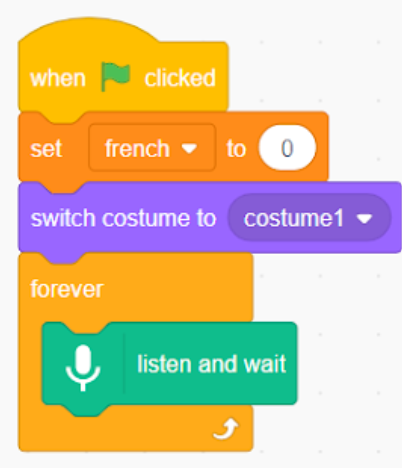
\includegraphics[width=6cm]{chapters/chapterCT1/figures/translate6.png}
    \caption{Code3}
    \label{fig:code3}
\end{figure}



Thank you to Machine Learning for Kids for creating such a brilliant Scratch extension - this is well worth a play with.


\part{Artificial Intelligence}
\usepackage{booktabs}


\chapter{Excel Neuron}
\section{Introduction}
Neural Networks, or more accurately artificial neural networks at their core a collection of simulated neurones. We can produce a simple neurone in Excel, that we can then get to learn a pattern and by repeating produce a simple neural network.

\section{Idea of a single artificial neuron}
At first, thinking about nerves and the brain may be at first a little scary - don't Panic. The neuron - the nerve cell - at basic level can be thought of a simple processing unit.

It has inputs these might be coming from other nerves or sensory input at this level we don't care really they are inputs and to start with the inputs are just going to be binary either 1 or 0. This is not as silly as it sounds in some nerves we either have the nerve firing (so a 1) or not firing (so a 0). This is simplistic but it a good starting point.
The neuron has an output again for all the examples in this chapter the output is going to be either 1 or 0.
The third part is the processing bit and this has two sub-parts. All the inputs are weighted, all this means is the particular input is multiplied to give a weighted value. As an example if the first input, let us call it X1 and it is 1, and the weight W1 is 0.1 then the weighted input is X1 x W1 =0.1. We do this for all the inputs and then we add all the weighted inputs together and produce a single number the weighted sum 0 first part done. The second part is taking the weighted sum and if the number is greater or equal to 0 then output is a 1 otherwise the output is 0.

One thing that we need to do is create a fake input X0=1 which is always 1 the weight W0 attached to it can change. For the moment please put up with this slightly strange thing - it is called a bias.

So, using figure 6.1 as our example
Weighted Sum = W0+W1.X1 +W2.X2 where . means times.
if Weighted Sum >=0 then Y(the output) =1 otherwise Y=0

So in the figure 6.1 example Weighted Sum = -1+X1+X2 (remember X1 and X2 can be 1 or 0). So to get an output (Y) to be 0 both X1 and X2 need to be 0 if one of then is a 1 then the output (y) is a 1. This is an OR gate. If we changed W0 from -1 to -2 then both X1 and X2 need to 1 to get a Y=1 - this is an AND gate.

The Big Secret: Change the weights we can get different functions from the 'neurone'.

\begin{figure}
    \centering
    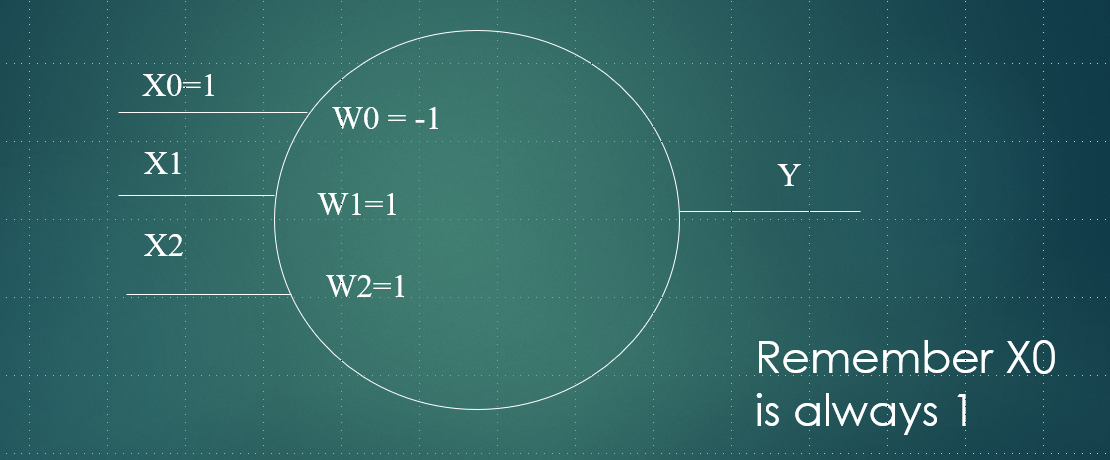
\includegraphics[width=10cm]{chapters/chAi1/figures/overall neurone2.png}
    \caption{Basic Artificial Neuron}
    \label{fig:basicneuron}
\end{figure}

\section{Building a Single Neuron}

On a blank sheet in either Excel or equivalent. 

1.  Write following headings 

A                B                            D                 E                 F                                      H                             J
X1	X2	 	W0	W1	W2	 	net 	 	Y

2.  Under X1 and X2 write down the four binary combinations - these are your inputs 

3   Under W0 W1 W2 write down three number W0 is the bias , W1 is the weight on input 1 and W2 is the weight on input 2

4 Under net on line 2 write this formula  =A2*$E$2+B2*$F$2+D2 and then copy and paste it into the next three cells below it.

5. Under Y type in the following  =IF(H2>=0,1,0)  and then copy and paste the formula to the three cells below it.


Hopefully it look similar to the one below.

\begin{tabular}{lllllll} \hline
X1 & X2 & W0 & W1 &	W2 & net & Y	 	 \\ \hline
0  & 0  & -2  & 1  & 1	 & 	-2 & 	0 \\ \hline
0  & 1	&     &    &     & 	-1 & 	0 \\ \hline  
1  & 0	&  	  &    & 	  & -1 & 	0 \\ \hline
1  & 1	& 	  &    &      &   0	 &  	1 \\ \hline
\end{tabular}

\newline
Questions

1 What logic operation has been carried out above?

2.If W0=1 W1=-1 and W2=-1  what logic operation do we have?

3. If W0=-1 W1=0 and W2=1  in terms of logic operation how else can be described Y in terms of X1 X2

4. Adjust the value of W0 (the bias) and then discuss with a colleague what do you think the main job of the bias is?

\section{Training a single neurone}
(i) Adapted the spreadsheet so that delta rule is used to train the neuron.
or
\newline
(ii) write a Python program that sets up a neurone, trains it and then test the neuron.
\newline
This is for those who want more of a challenge in the class
\newline
\newline
In both you will need to the following:
\newline
(i) Set X0, X1, X2 up and cycle through each input combination;
\newline
(ii) Set some weights;
\newline
(iii) Calculated net and then get the output of the neuron as before.
\newline
(iv) The error = Desired output - actual output and set the eta/learning coefficient to 0.5
\newline
(v) for each weight workout the change in the weight (delta rule) = (input connected to the weight)*(learning coefficient)*(Error)
\newline
(vi) Add the change in the weights to the old weights to give the new weight
\newline
(vii) For each combination repeat (iii) to (vi)
\newline
(vii) Repeat (vii) until for every input the error =0 
\UrlBigBreaks{}

\section{Reflection and Feedback}
Now try to get your system to find the weights for the following

\begin{tabular}{lll} \hline
X1 & X2 & Output	 	 \\ \hline
0  & 0  & 0 \\ \hline
0  & 1	& 1 \\ \hline  
1  & 0	& 1 \\ \hline
1  & 1	& 0 \\ \hline
\end{tabular}

What happened? Why?

\section{Three neurones connect - we have a network}
Using what you learnt from the previous sections we can build three neurones
\newline
First building a neurone in the Spreadsheet to give the following output (output 1)
\begin{tabular}{lll} \hline
X1 & X2 & Output1	 	 \\ \hline
0  & 0  & 0 \\ \hline
0  & 1	& 0 \\ \hline  
1  & 0	& 1 \\ \hline
1  & 1	& 0 \\ \hline
\end{tabular}
\newline
Next building another neurone in the same Spreadsheet to give the following output (output 2)
\begin{tabular}{lll} \hline
X1 & X2 & Output2	 	 \\ \hline
0  & 0  & 0 \\ \hline
0  & 1	& 1 \\ \hline  
1  & 0	& 0 \\ \hline
1  & 1	& 0 \\ \hline
\end{tabular}

Now create a third neuron that instead of using inputs X1 and X2 uses the outputs output 1 and output 2 as its inputs and produces the following:
\begin{tabular}{lll} \hline
output 1 & output 2 & Final Output	 	 \\ \hline
0  & 0  & 0 \\ \hline
0  & 1	& 1 \\ \hline  
1  & 0	& 0 \\ \hline
1  & 1	& 0 \\ \hline
\end{tabular}
When its is built what should happen we have have combined the outputs from the first two neurons as inputs to another neurons. We have a network of neurons or a Neural Network!
\newline 
When X1 and X2 varies as below the final Output should work now.
\begin{tabular}{lll} \hline
output 1 & out 2 & Final Output	 	 \\ \hline
0  & 0  & 0 \\ \hline
0  & 1	& 1 \\ \hline  
1  & 0	& 1 \\ \hline
1  & 1	& 0 \\ \hline
\end{tabular}

\chapter{Microbit Neural Network - python}

\section{without the microbit}
\subsection{Overview:}
The characteristics of the system will be:
Inputs are going to be binary
Weighted sum is bias+W1*input1+w2*input2
If weighted sum>=0 then the output is True (T on the LEDs) or '1'
If weighted sum<0 then the output is False (F on the LEDs) or '0

subsection{Single Neuron (without the Microbit)}
Lets start without the microbit and build a single neuron in Python and useful exercise in it's own right just to see the mechanism. A class Neuron is produced and all possible combination of a two-input binary system are feed in. 
\begin{verbatim}
class Neuron:
    def __init__(self, input1, bias, w1, w2):
        self.input1 = input1
        self.bias = bias
        self.w1=w1
        self.w2=w2
    
    def CalculateOutput (self):
        output1 = 0
        net = self.bias+self.input1[0]*self.w1+self.input1[1]*self.w2
        if net >= 0:
            output1 = 1
        else:
            output1 = 0
        return output1


for x1 in range (2):
    for x2 in range (2):
        neuron1= Neuron([x1,x2],-1,1,1)

        print("x1="+str(x1)+"x2= "+str(x2)+" Output= " +str(neuron1.CalculateOutput()))
\end{verbatim}


The code above implements a simple single neuron and the weights -1,1,1 produce an OR gate and -2,1,1 produces an AND gate.

\subsection{A Neural Network}
We can extend the code above to produce a neural network, by feeding the outputs of one or more neurons as inputs to other neurones. The code below produces an Exclusive XOR - essentially for the two input case if the two inputs are different then the output is True. The same inputs go to two neurones but they have different weight (bias, W1 and W2) but the outputs from these neurones are the inputs to a third neurone. The code is shown below (the Neuron class hasn't changed):
\begin{verbatim}
    class Neuron:
    def __init__(self, input1, bias, w1, w2):
        self.input1 = input1
        self.bias = bias
        self.w1=w1
        self.w2=w2
    
    def CalculateOutput (self):
        output1 = 0
        net = self.bias+self.input1[0]*self.w1+self.input1[1]*self.w2
        if net >= 0:
            output1 = 1
        else:
            output1 = 0
        return output1


for x1 in range (2):
    for x2 in range (2):
        neuron1= Neuron([x1,x2],-1,-1,1)
        neuron2= Neuron([x1,x2],-1,1,-1)
        neuron3= Neuron([neuron1.CalculateOutput(),neuron2.CalculateOutput()],-1,1,1)
        print("x1="+str(x1)+"x2= "+str(x2)+" Output 1= "+str(neuron1.CalculateOutput())+" Output 2= "+str(neuron2.CalculateOutput())+" Output overall= "+str(neuron3.CalculateOutput()))
\end{verbatim}


        



\section{with the microbit}
This is second in a two-post series on building a neural network using microbits with micropython. 
In the first post python was used to produce a neural network without the microbits. 

In this post the network is as shown in figure 1 is developed.

The figure below shows the arrangement of the connections to be built; pin 2 is the output of each neuron. 

The two micro:bits/neurons on the left of the picture taking in the two same inputs; the output from these neurons are the two inputs to the output neuron on the right.

The micro:bit objects used in Figure 1 were produced using the micro:bit Fritzing diagram available at 
\url{https://github.com/microbit-foundation/dev-docs/issues/36} thanks to David Whale (@whalleygeek ) for this.

\begin{figure}
    \centering
    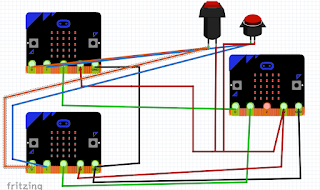
\includegraphics[width=10cm]{chapters/chAi1/figures/Screen Shot 2018-04-03 at 14.08.07.png}
    \caption{Microbit neural network}
    \label{fig:MicroibitANN1}
\end{figure}

\section{The Inputs neurons}

Neuron 1:

\begin{verbatim}
from microbit import *
W=[-1,-1,1]
while True:
    x1=pin0.read_digital()
    x2=pin1.read_digital()
    net = W[0]+W[1]*x1+W[2]*x2
    if net>=0:
        display.scroll("T")
        pin2.write_digital(1)
    else:
        display.scroll("F")
        pin2.write_digital(0)
\end{verbatim}


Neuron 2
\begin{verbatim}
from microbit import *
W=[-1,1,-1]
while True:
    x1=pin0.read_digital()
    x2=pin1.read_digital()
    net = W[0]+W[1]*x1+W[2]*x2
    if net>=0:
        display.scroll("T")
        pin2.write_digital(1)
    else:
        display.scroll("F")
        pin2.write_digital(0)   
\end{verbatim}




\section{Output Neuron.}
Feeding the inputs from Neuron 1 and Neuron 2 as inputs

\begin{verbatim}
from microbit import *
W=[-1,1,1]
while True:
    x1=pin0.read_digital()
    x2=pin1.read_digital()
    net = W[0]+W[1]*x1+W[2]*x2
    if net>=0:
        display.scroll("T")
        pin2.write_digital(1)
    else:
        display.scroll("F")
        pin2.write_digital(0)  
\end{verbatim}







\chapter{TinkerCad for Microbit Neural Network}
\section{Introduction}
\section{Single neurone in tinkerCad}
The free online CAD (and so much more) package Tinkercad \url{https://www.tinkercad.com/} under circuits; now has microbits as part of the list of basic components available to build circuits out of.
\begin{figure}
    \centering
    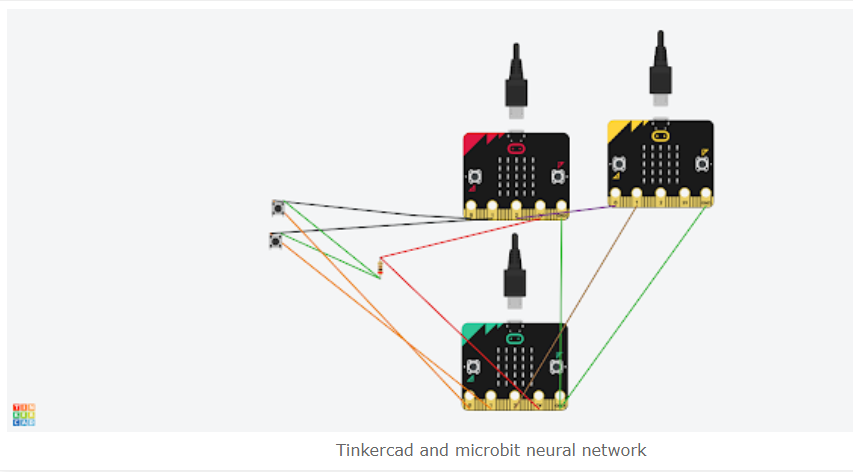
\includegraphics[width=11cm]{chapters/chAi1/figures/Tinkercadann1.png}
    \caption{TinkerCad Microbit Network}
    \label{fig:tinkercad_neural_microbit_network}
\end{figure}
To have a quick play I wonder if using the built in Scratch-like code blocks, I could build a simulation of neuron on the microbit.

Requirements 
- By altering the bias, weights change the behaviour of buttons A and B
-when A is pressed a variable input1 is set to 1 and when released it goes to 0. The same happens for Button B and a variable input 2
- if (bias+weight1*input1+weight2*input2)>=0 then a T for True appears of the LEDs otherwise F for False is shown.
\begin{figure}
    \centering
    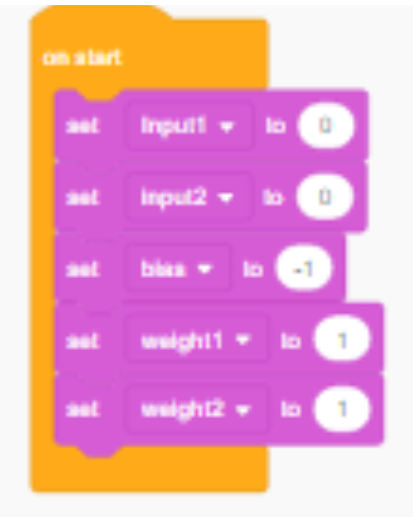
\includegraphics[width=11cm]{chapters/chAi1/figures/Tinkercadann2.png}
    \caption{TinkerCad Microbit Network: setting up}
    \label{fig:tinkercad_neural_microbit_network_basic}
\end{figure}
That is it really, apart initialising the variables. The code for producing an OR is shown below and the GIF at the end shows an AND in action:
\begin{figure}
    \centering
    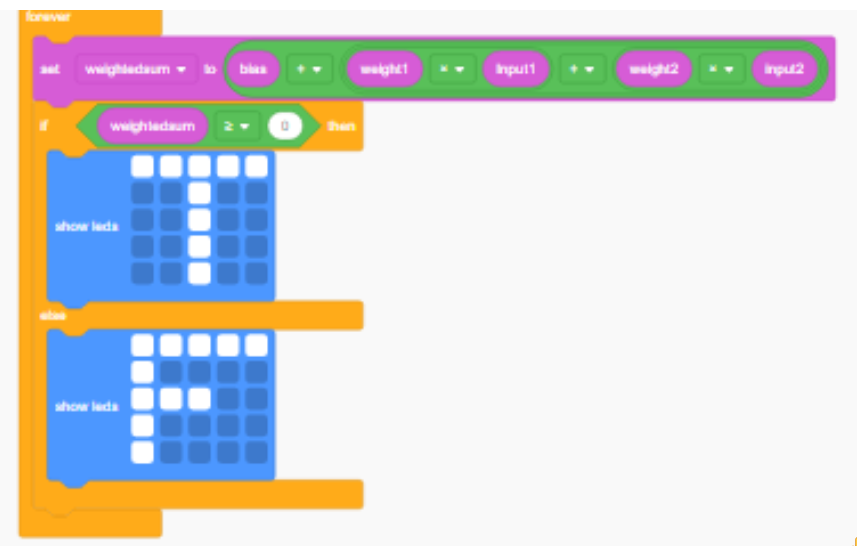
\includegraphics[width=11cm]{chapters/chAi1/figures/Tinkercadann23.png}
    \caption{TinkerCad Microbit Network: basic unit}
    \label{fig:tinkercad_neural_microbit_network_basic2}
\end{figure}
The so in action for an AND (bias is set to -2); change the bias to -1 and you would get an OR.

\begin{figure}
    \centering
    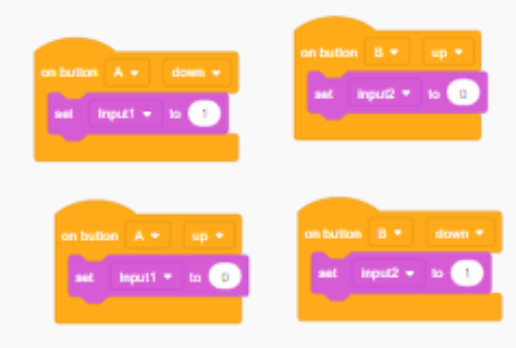
\includegraphics[width=11cm]{chapters/chAi1/figures/Tinkercadann4.png}
    \caption{TinkerCad Microbit Network: }
    \label{fig:tinkercad_neural_microbit_network_basic3}
\end{figure}

The whole thing is available at: \url{https://www.tinkercad.com/things/8Ph6UBFdICz-brave-duup }

Originally published at \url{https://robotsandphysicalcomputing.blogspot.com/2021/01/tinkercad-and-microbit-to-make-neuron.html}


\section{Microbit neural network with TinkerCad}
In a previous post I produced a single neuron based around microbits in Tickercad - see here.

To extend this the basic ideas discussed in that the previous post where extended to three microbit joined together. In  other words a network of neurones or neural network.

Basic requirements of a neuron are
Requirements 
- By altering the bias (or w0 in the example), weights change the behaviour of switches changes.
-when switch is pressed a variable x1 or x2 is set to 1 depending on which button is pressed and when released it goes to 0. 
- if (bias+w1*x1+w2*x2)>=0 then a T for True appears of the LEDs otherwise F for False is shown.

So by selecting the weights and connecting the outputs (p2) from the microbits labelled as Red and Green in the image above as inputs to the yellow microbit 'neuron' we can form a neural network. Switches as the inputs and the screen on the yellow 'neuron' as the output of the network showing true (T) or false(F).

So to build a XOR from the 'neurons'
'hidden layer'
Red microbit had the variables w0 set to -1 and W1 set to 0 and W2 set 1
Green microbit had the variables w0 set to -1 and W1 set to 1 and W2 set 0

'output layer'
Yellow microbit had the variables w0 set to -1 and W1 set to 1 and W2 set 1

All of this can be found at https://www.tinkercad.com/things/hPV4nU0Asr5-smooth-bojo or through the link shown below:

Originally published at \url{https://robotsandphysicalcomputing.blogspot.com/2021/02/making-neural-network-in-tinkercad-from.html}


\bibliography{}
\bibliographystyle{plain}
Barr, D., Harrion, J., and Conery, L. (2011) Computational Thinking: A Digital Age Skill for Everyone Leading and Learning with Technology, ISTE, March/April 2011 [accessed via http://www.csta.acm.org/Curriculum/sub/CurrFiles/LLCTArticle.pdf on 26/12/2015]
 
Barr, V. and Stephenson, C. (2011) Bringing Computational Thinking to K-12, ACM Inroads, Vol 2. No 1, pp 48 - 54 [accessed via http://csta.acm.org/Curriculum/sub/CurrFiles/BarrStephensonInroadsArticle.pdf on 26/12/2015]
https://doi.org/10.1145/1929887.1929905
 
Computing at School (2013) Computing in the National Curriculum: A guide for primary teachers [accessed via http://www.computingatschool.org.uk/data/uploads/CASPrimaryComputing.pdf on 13/3/2016]
 
Denning, Peter J. (2009) Beyond Computational Thinking, Communications of the ACM Vol 52, Issue 6, pp 28 - 30 [accessed via http://sgd.cs.colorado.edu/wiki/images/7/71/Denning.pdf on 26/12/2015]
 
DfE: Department for Education (2013) National Curriculum in England: computing programmes of study
 
Freedman, J. (2015) Cycloid Drawing Machine [online] URL: https://www.kickstarter.com/projects/1765367532/cycloid-drawing-machine accessed on 3/3/2016.
 
Google. 2016 Project Jacquard [online] URL: https://www.google.com/atap/project-jacquard/ accesed on:1/3/2016.
 
Knuth, D. 1968. Preface, The Art of Programming vol 1., Boston: Addison-Wesley.
 
Knuth, D. 1996. Foreword. In: Petkovsek, M., Wilf, H., Zeilberger, D. A=B.. Natick: A K Peters/CRC Press, vii.
 
Koetsier, T., 2001. On the prehistory of programmable machines: Musical automata, looms, calculators. Mechanism and Machine Theory, 36(5), 589-603.
https://doi.org/10.1016/S0094-114X(01)00005-2
 
Menegus, B (2016) CDMS: Built with Processing [online] URL: http://wheelof.com/sketch/ accessed on 4/3/2016
 
MoMA. 2012. MoMA| Video Games [online] URL: http://www.moma.org/explore/inside_out/2012/11/29/video-games-14-in-the-collection-for-starters/ accessed on: 1/3/2016.
 
Papert, S (1993) The children's machine: Rethinking schools in the age of the computer. New York: Basic books
 
Pearson M (2011) Generative Art: A practical guide using Processing, New York: Manning, 3-12
 
Selby, C. and Woollard, J. (2013) Computational thinking: the developing definition University of Southampton [accessed via http://eprints.soton.ac.uk/356481/7/Selby_Woollard_bg_soton_eprints.pdf on 26/12/2015]
 
The Art Story (2016) Sol LeWitt [online] http://www.theartstory.org/artist-lewitt-sol.htm accessed on: 6/3/2016
 
Wing, J. (2006) Computational Thinking Communications of the ACM Vol 49 pp 33 - 35 [accessed via https://www.cs.cmu.edu/~15110-s13/Wing06-ct.pdf on 26/12/2015]
https://doi.org/10.1145/1118178.1118215
 
Wing, J. (2011) Computational Thinking - What and Why The Link - News from the School of Computer Science, Issue 6.0, Spring 2011 [accessed via http://www.cs.cmu.edu/sites/default/files/11-399_The_Link_Newsletter-3.pdf on 26/12/2015]
 
Liukas L (2015) Activity 7 The Robots Hello Ruby - Adventures in Coding, New York: Feiwel and Friends, 94-97.
 
Schofield, S (2016) Generative Artworks [online] URL: http://www.simonschofield.net
 
Turner S (2016) 3 'Art' Scratch Projects [online] URL: http://compuationalthinking.blogspot.co.uk/2016/03/3-of-my-scratch-projects-for-week.html accessed on: 12/3/2016.

\printindex

\end{document}
